
%%%%%%%%%%%%%%%%%%%%%%%%%%%%%%%%%%%%%%%%%%%%%%%%%%%%%%%%%%%%%%%%%%
% Sample template for MIT Junior Lab Student Written Summaries
% Available from http://web.mit.edu/8.13/www/Samplepaper/sample-paper.tex
% Last Updated April 12, 2007
% Adapted from the American Physical Societies REVTeK-4 Pages
% at http://publish.aps.org
%\newcommand{\mjmlegacy}{}

\setlength{\paperheight}{11in}
% http://tex.stackexchange.com/questions/74636/mla-package-and-thumbpdf
\makeatletter
\@namedef{ver@thumbpdf.sty}{}
\makeatother




\ifdefined\mjmlegacy
\documentclass[aps,secnumarabic,balancelastpage,amsmath,amssymb,nofootinbib]{revtex4}
\else
\documentclass[aps,secnumarabic,balancelastpage,amsmath,amssymb,nofootinbib]{revtex4-2}
\usepackage{array}[=2016-10-06]
\fi


%http://tex.stackexchange.com/questions/119905/insert-multiple-figures-in-latex

\usepackage[nomessages]{fp}    %mjm   needed for chemfig and mol2chemfig computed angles  
\usepackage{siunitx}        %mjm  appendix table subsections  
%\usepackage{morefloats}        %mjm   saving up figs for the end   
% fking incompatibvle fuxk ing floatrow 
%\usepackage{float}        %mjm  appendix table subsections  
\usepackage{pbox}        %mjm box off junk  
\usepackage{comment}        %mjm  see the build options  
\usepackage{framed}        %mjm box off junk  
\usepackage{lgrind}        % convert program listings to a form includable in a LaTeX document
% comment out for biblatex test
% causes problems on texlive 2023+
%\usepackage{chapterbib}    % allows a bibliography for each chapter (each labguide has it's own)
%\usepackage{biblatex}   
\usepackage{color}         % produces boxes or entire pages with colored backgrounds
\usepackage{graphics}      % standard graphics specifications
\usepackage[pdftex]{graphicx}      % alternative graphics specifications
%\usepackage{graphicx}      % alternative graphics specifications
\usepackage{longtable}     % helps with long table options
\usepackage{epsf}          % old package handles encapsulated post script issues
\usepackage{bm}            % special 'bold-math' package
\usepackage{url}            % path for stupid jobname   
%\usepackage{asymptote}     % For typesetting of mathematical illustrations
\usepackage{thumbpdf}
\usepackage[colorlinks=true]{hyperref}  % this package should be added after all others
%\usepackage[draft=false, x-bib-pages=\input{\mjmbasename.last_page}, colorlinks=true]{hyperref}  % this package should be added after all others
%\usepackage[draft=false, x-bib-pages=\input{allbib.last_page}, colorlinks=true]{hyperref}  % this package should be added after all others
                                        % use as follows: \url{http://web.mit.edu/8.13}

%http://tex.stackexchange.com/questions/12676/add-notes-under-the-table
%\usepackage{booktabs,caption,fixltx2e}
% not work with subfig????
\usepackage[CaptionAfterwards]{fltpage}
\usepackage{lipsum}

% this does not  work .... 
%\usepackage[utf8]{inputenc}
%\usepackage{tabulary}
\usepackage[para,online,flushleft]{threeparttable}
%\usepackage{threeparttable}

%\usepackage{chemfig}
\usepackage[version=3]{mhchem}        %  
\usepackage{mol2chemfig}
% chemfig vriables maybe
\usepackage{xstring}        %mjm  appendix table subsections  
%\usepackage{chemformula}
% \usepackage{chemmacros}
\usepackage{floatrow}
\usepackage{fancyhdr}
%  underscore in jobmane f 
% https://latex.org/forum/viewtopic.php?t=2975
% this also messes up pdftotext  
%\usepackage[T1]{fontenc}
\usepackage{dcolumn} % https://tex.stackexchange.com/questions/2746/aligning-numbers-by-decimal-points-in-table-columns

\usepackage{catchfile} % mjmaddbib needs to read page count file
\pagestyle{fancy}




\newcolumntype{.}[1]{D{.}{.}{#1}}
%\usepackage[maxfloats=30]{morefloats}   %mjm   saving up figs for the end   
% no param on old version stuck at 36
\usepackage{morefloats}        %mjm   saving up figs for the end   
\usepackage{graphicx}        %mjm   saving up figs for the end   

% will need modificaitons 

% 2020-10-18 extract some new boilerplate 

% https://tex.stackexchange.com/questions/121601/automatically-wrap-the-text-in-verbatim
\usepackage{listings}
\lstset{
basicstyle=\small\ttfamily,
columns=flexible,
breaklines=true
}
%%%%%%%%%%%%%%%%%%%%%%%%%%%%% utilitites

\newcommand{\mjmblackbox}[2]{
 \fbox{
% thi does not ing work right 
\begin{minipage}[t]{\textwidth}
{ \centering{\bf{#1 : }} }
\par
#2
\end{minipage}
}
}
\newcommand{\mjmblackboxno}[2]{
 \fbox{
% thi does not ing work right 
\begin{minipage}[t]{\textwidth}
{ \centering{\bf{#1 : }} }
#2
\end{minipage}
}
}





%%%%%%%%%%%%%%%%%%%%%%%% biblio stuff



\newcommand{\checkrel}[1]{%
  \ifcsname#1\endcsname%
\newcommand{\mjmstatus}{  public NOTES }
\newcommand{\mjmversion}{\mjmrelease}
  \else%
\newcommand{\mjmstatus}{ NOT public NOTES }
\newcommand{\mjmversion}{0.00}
  \fi%
}




% https://tex.stackexchange.com/questions/18089/are-there-any-command-for-producing-the-bibtex-logo
%\def\BibTeX{{\rm B\kern-.05em{\sc i\kern-.025em b}\kern-.08em
%    T\kern-.1667em\lower.7ex\hbox{E}\kern-.125emX}}

\newcommand{\biblogo}{
{{\rm B\kern-.05em{\sc i\kern-.025em b}\kern-.08em
    T\kern-.1667em\lower.7ex\hbox{E}\kern-.125emX}}
{ }  }
%\newcommand{\biblogo}{ Bibte{\it X}  { }  }
\newcommand{\latexlogo}{ \LaTeX  { }  }
\newcommand{\bomtexlogo}{ BomTe{\it X}  { }  }






\newcommand{\mjmvirus}{SARS-Cov-2 }
\newcommand{\mjmdisease}{covid-19 }
\newcommand{\Mjmdisease}{Covid-19 }
\newcommand{\mjmlogo}{ MUQED { }  }
\newcommand{\mjmlinkedin}{ {\bf LinkedIn} { }  }








% https://tex.stackexchange.com/questions/121601/automatically-wrap-the-text-in-verbatim
\usepackage{listings}
\lstset{
basicstyle=\small\ttfamily,
columns=flexible,
breaklines=true
}

% none of this fking fking works for a f F 
\newcommand{\mjmverbatim}{lstlisting}
\newcommand{\mjmbeginverbatim}{\begin{lstlisting}}
\newcommand{\mjmendverbatim}{\end{lstlisting}}

\newcommand{\mjmmangle}[1]{keep/#1}




\usepackage[section]{placeins}

%\ifdefined\mjmlegacy
%\documentclass[aps,secnumarabic,balancelastpage,amsmath,amssymb,nofootinbib]{revtex4-2}
%\else
%\documentclass[aps,secnumarabic,balancelastpage,amsmath,amssymb,nofootinbib]{revtex4} \fi

%http://tex.stackexchange.com/questions/119905/insert-multiple-figures-in-latex

\usepackage[nomessages]{fp}    %mjm   needed for chemfig and mol2chemfig computed angles  
\usepackage{siunitx}        %mjm  appendix table subsections  
%\usepackage{morefloats}        %mjm   saving up figs for the end   
% fking incompatibvle fuxk ing floatrow 
%\usepackage{float}        %mjm  appendix table subsections  
\usepackage{pbox}        %mjm box off junk  
\usepackage{comment}        %mjm  see the build options  
\usepackage{framed}        %mjm box off junk  
\usepackage{lgrind}        % convert program listings to a form includable in a LaTeX document
% comment out for biblatex test
% causes problems on texlive 2023+
%\usepackage{chapterbib}    % allows a bibliography for each chapter (each labguide has it's own)
%\usepackage{biblatex}   
\usepackage{color}         % produces boxes or entire pages with colored backgrounds
\usepackage{graphics}      % standard graphics specifications
\usepackage[pdftex]{graphicx}      % alternative graphics specifications
%\usepackage{graphicx}      % alternative graphics specifications
\usepackage{longtable}     % helps with long table options
\usepackage{epsf}          % old package handles encapsulated post script issues
\usepackage{bm}            % special 'bold-math' package
\usepackage{url}            % path for stupid jobname   
%\usepackage{asymptote}     % For typesetting of mathematical illustrations
\usepackage{thumbpdf}
\usepackage[colorlinks=true]{hyperref}  % this package should be added after all others
%\usepackage[draft=false, x-bib-pages=\input{\mjmbasename.last_page}, colorlinks=true]{hyperref}  % this package should be added after all others
%\usepackage[draft=false, x-bib-pages=\input{allbib.last_page}, colorlinks=true]{hyperref}  % this package should be added after all others
                                        % use as follows: \url{http://web.mit.edu/8.13}

%http://tex.stackexchange.com/questions/12676/add-notes-under-the-table
%\usepackage{booktabs,caption,fixltx2e}
% not work with subfig????
\usepackage[CaptionAfterwards]{fltpage}
\usepackage{lipsum}

% this does not  work .... 
%\usepackage[utf8]{inputenc}
%\usepackage{tabulary}
\usepackage[para,online,flushleft]{threeparttable}
%\usepackage{threeparttable}

%\usepackage{chemfig}
\usepackage[version=3]{mhchem}        %  
\usepackage{mol2chemfig}
% chemfig vriables maybe
\usepackage{xstring}        %mjm  appendix table subsections  
%\usepackage{chemformula}
% \usepackage{chemmacros}
\usepackage{floatrow}
\usepackage{fancyhdr}
%  underscore in jobmane f 
% https://latex.org/forum/viewtopic.php?t=2975
% this also messes up pdftotext  
%\usepackage[T1]{fontenc}
\usepackage{dcolumn} % https://tex.stackexchange.com/questions/2746/aligning-numbers-by-decimal-points-in-table-columns

\usepackage{catchfile} % mjmaddbib needs to read page count file
\pagestyle{fancy}




\newcolumntype{.}[1]{D{.}{.}{#1}}
%\usepackage[maxfloats=30]{morefloats}   %mjm   saving up figs for the end   
% no param on old version stuck at 36
\usepackage{morefloats}        %mjm   saving up figs for the end   
\usepackage{graphicx}        %mjm   saving up figs for the end   

% will need modificaitons 
%
% 2020-10-18 extract some new boilerplate 

% https://tex.stackexchange.com/questions/121601/automatically-wrap-the-text-in-verbatim
\usepackage{listings}
\lstset{
basicstyle=\small\ttfamily,
columns=flexible,
breaklines=true
}
%%%%%%%%%%%%%%%%%%%%%%%%%%%%% utilitites

\newcommand{\mjmblackbox}[2]{
 \fbox{
% thi does not ing work right 
\begin{minipage}[t]{\textwidth}
{ \centering{\bf{#1 : }} }
\par
#2
\end{minipage}
}
}
\newcommand{\mjmblackboxno}[2]{
 \fbox{
% thi does not ing work right 
\begin{minipage}[t]{\textwidth}
{ \centering{\bf{#1 : }} }
#2
\end{minipage}
}
}





%%%%%%%%%%%%%%%%%%%%%%%% biblio stuff



\newcommand{\checkrel}[1]{%
  \ifcsname#1\endcsname%
\newcommand{\mjmstatus}{  public NOTES }
\newcommand{\mjmversion}{\mjmrelease}
  \else%
\newcommand{\mjmstatus}{ NOT public NOTES }
\newcommand{\mjmversion}{0.00}
  \fi%
}




% https://tex.stackexchange.com/questions/18089/are-there-any-command-for-producing-the-bibtex-logo
%\def\BibTeX{{\rm B\kern-.05em{\sc i\kern-.025em b}\kern-.08em
%    T\kern-.1667em\lower.7ex\hbox{E}\kern-.125emX}}

\newcommand{\biblogo}{
{{\rm B\kern-.05em{\sc i\kern-.025em b}\kern-.08em
    T\kern-.1667em\lower.7ex\hbox{E}\kern-.125emX}}
{ }  }
%\newcommand{\biblogo}{ Bibte{\it X}  { }  }
\newcommand{\latexlogo}{ \LaTeX  { }  }
\newcommand{\bomtexlogo}{ BomTe{\it X}  { }  }






\newcommand{\mjmvirus}{SARS-Cov-2 }
\newcommand{\mjmdisease}{covid-19 }
\newcommand{\Mjmdisease}{Covid-19 }
\newcommand{\mjmlogo}{ MUQED { }  }
\newcommand{\mjmlinkedin}{ {\bf LinkedIn} { }  }








% https://tex.stackexchange.com/questions/121601/automatically-wrap-the-text-in-verbatim
\usepackage{listings}
\lstset{
basicstyle=\small\ttfamily,
columns=flexible,
breaklines=true
}

% none of this fking fking works for a f F 
%mjmlegacy
%\newcommand{\mjmverbatim}{lstlisting}
%\newcommand{\mjmbeginverbatim}{\begin{lstlisting}}
%\newcommand{\mjmendverbatim}{\end{lstlisting}}

%\newcommand{\mjmmangle}[1]{keep/#1}




%# CHANGE VERSION AND STATUS MANUALLY 
% need a draft/notes/release flag

% https://tex.stackexchange.com/questions/5894/latex-conditional-expression
%At the command-line, you can do \def\MYFLAG{} and then test if \MYFLAG is defined in your document (or an included style file) with \ifdefined\MYFLAG ... \else ... \fi.
% needs trailing space for the sample bibtex doh
% leading spaces mess up the entry thought 
\def\xxmjmrelease{0.10 }
\ifdefined\mjmrelease
\newcommand{\mjmstatus}{ PUBLIC NOTES }
\newcommand{\mjmversion}{\mjmrelease} %%%%%%%%%%%%%
\newcommand{\mjmtrno}{MJM-2025-002}
\newcommand{\mjmbib}{\mjmtrno-\mjmversion}
\newcommand{\mjmstatuswarn}{{\bf{  }}   }
% 2021-09-29 wanted version wth for brownie
%\newcommand{\mjmbib}{\mjmtrno-\mjmversion-\mjmrelease}
%\newcommand{\mjmbib}{\mjmtrno}
\else
\newcommand{\mjmstatus}{ NOT public NOTES }
\newcommand{\mjmversion}{0.00} %%%%%%%%%%%%%
\newcommand{\mjmtrno}{MJM-2025-002}
%\newcommand{\mjmbib}{\mjmtrno-\mjmversion}
\newcommand{\mjmbib}{\mjmtrno}
%\newcommand{\mjmstatuswarn}{  }
\newcommand{\mjmstatuswarn}{{\bf{This document is a non-public DRAFT and contents may be speculative or undocumented or simple musings and should be read as such.  }}   }
\fi

%\newcommand{\mjmstatus}{ NOT public NOTES }



\newcommand{\mjmtitle}{EUV Lithography : Don't take my kodachrome away}
\begin{comment}
\newcommand{\xxmjmmakedate}{ }
\newcommand{\xxmjmauthor}{Mike J Marchywka }
\newcommand{\xxmjmbasename}{\jobname}
\newcommand{\xxmjmaddbio}{mjm_tr,releases}
\newcommand{\xxmjmversion}{ 0.00 }
\newcommand{\xxmjmtrno}{MJM-2018-009}
\newcommand{\xxmjmbibday}{12}
\newcommand{\xxmjmbibmo}{12}
\newcommand{\xxmjmbibyear}{2018}
\newcommand{\xxmjmemail}{marchywka@hotmail.com}
\end{comment}



\ifdefined\mjmlegacy
\newcommand{\expandableinput}[1]{\input{#1}}
\else
% https://tex.stackexchange.com/questions/583927/misplaced-noalign-error-with-input-in-a-table-after-the-2020-fall-latex-releas/583939#583939
\ExplSyntaxOn % providing \expandableinput
\cs_new:Npn \expandableinput #1
  { \use:c { @@input } { \file_full_name:n {#1} } }
\ExplSyntaxOff
\fi



\ifdefined\grad
\else
\newcommand{\grad}{\nabla}
\fi
\newcommand{\mjmquote}[1]{{\centering {\it #1 }}}
\newcommand{\mjmwisdom}[1]{{\centering {\it #1 }}}
\newcommand{\laplace}{\nabla^{2}}
\newcommand{\mjmdx}[2]{\left(\frac{\partial #1 }{\partial #2} \right) }
\newcommand{\mjmdxop}[2]{\frac{\partial  }{\partial #2}\left( #1 \right) }
\newcommand{\mjmdxdx}[2]{\left(\frac{\partial^{2} #1 }{\partial #2^{2}} \right) }
\newcommand{\mjmdxo}[2]{\frac{\partial #1 }{\partial #2} }
\newcommand{\mjmdxx}[2]{\left(\frac{\partial^{2} #1 }{\partial {#2}^{2}} \right) }
\newcommand{\mjmD}[3]{\frac{d^{#1} #2 }{d{#3}^{#1}}  }
\newcommand{\mjmDnt}[2]{\frac{d^{#1} #2 }{dt^{#1}}  }
\newcommand{\mjmDparen}[2]{ {#1}^{(#2)} }
\newcommand{\mjmdxy}[3]{\left(\frac{\partial^{2} #1 }{\partial {#2}\partial{#3}} \right) }
\newcommand{\mjmdxyn}[5]{\left(\frac{\partial^{#1} }{\partial^{#2} {#3}\partial^{#4}{#5}} \right) }
\newcommand{\mjmdsq}[2]{\left(\frac{\partial #1 }{\partial #2} \right) ^{2}}
\newcommand{\mjmupdated}[2]{\p  Updated on $#1$ from source #2 \p }
% see tug mail archives, based on discussion 
%\bool_new:N \l_tmpa_bool
\newif\ifbibstarted
\newif\ifbibnamed
\bibstartedfalse
\bibnamedfalse
\newcommand{\mjmtotalbib}{}
%\def\foo{}
\newcommand{\mjmsummabib}[2]{
%\renewcommand{\mjmtotalbib}{ \mjmtotalbib, #1 = #2 }
%\let\foo{ #1 = #2}
}
%%%%%%%%%%%%%%%%%%%%%%%%%%%%%%%%%%%%%%%%%%%%%%%%%%%%%%%%%%%%%%%%

\iffalse
@software{,
  author = {Michael J Marchywka},
  city = {Jasper GA 30143 USA},
  title = { A one-file library for adding machine and human readable bibtex to an article },
abstract={ A simple include file to make bibtex available 
in a document in both machine and human readable format. 
Machine readable is added to extended information 
which can be read with tools such as exiftool ( https://exiftool.org/ ).
While typically not complete at time of pdf creation,
other tools such as toobib can be used to complete the citation
and of course publishers may be able to modify it too as 
more is known. The human readable form need not beincluded
in document types not suited for that but then automated citation
may still be easy.  
See also some exchanges on the Texhax mailing list @tug.org },
institution={},
license={Knowledge sir should be free to all },
publisher={Mike Marchywka},
email={marchywka@hotmail.com},
authorid={orcid.org/0000-0001-9237-455X},
  filename = {mjmaddbib.tex},
  url = {},
  version = {0.0.0},
  date-started = {}
}

<one line to give the program's name and a brief idea of what it does.>


Conceived and written by Mike Marchywka from 2019 to present.
See dates in individual code pieces as they were 
generated from my wizards. 
Copyright (C) <year> <name of author>


This program is free software: you can redistribute it and/or modify it under
the terms of the GNU General Public License as published by the Free Software
Foundation, either version 3 of the License, or (at your option) any later
version.

This program is distributed in the hope that it will be useful, but WITHOUT ANY
WARRANTY; without even the implied warranty of  MERCHANTABILITY or FITNESS FOR
A PARTICULAR PURPOSE. See the GNU General Public License for more details.

You should have received a copy of the GNU General Public License along with
this program.  If not, see <http://www.gnu.org/licenses/>.

   THIS SOFTWARE IS PROVIDED BY THE COPYRIGHT HOLDERS AND CONTRIBUTORS
   "AS IS" AND ANY EXPRESS OR IMPLIED WARRANTIES, INCLUDING, BUT NOT
   LIMITED TO, THE IMPLIED WARRANTIES OF MERCHANTABILITY AND FITNESS FOR
   A PARTICULAR PURPOSE ARE DISCLAIMED.  IN NO EVENT SHALL THE COPYRIGHT OWNER OR
   CONTRIBUTORS BE LIABLE FOR ANY DIRECT, INDIRECT, INCIDENTAL, SPECIAL,
   EXEMPLARY, OR CONSEQUENTIAL DAMAGES (INCLUDING, BUT NOT LIMITED TO,
   PROCUREMENT OF SUBSTITUTE GOODS OR SERVICES; LOSS OF USE, DATA, OR
   PROFITS; OR BUSINESS INTERRUPTION) HOWEVER CAUSED AND ON ANY THEORY OF
   LIABILITY, WHETHER IN CONTRACT, STRICT LIABILITY, OR TORT (INCLUDING
   NEGLIGENCE OR OTHERWISE) ARISING IN ANY WAY OUT OF THE USE OF THIS
   SOFTWARE, EVEN IF ADVISED OF THE POSSIBILITY OF SUCH DAMAGE.


\fi

%\usepackage[pdftex]{graphicx}      % alternative graphics specifications
\usepackage{hyperref}      %


\newcommand{\mjmstartbib}[2]
{
\def\mjmbibentry{@#1\{#2}
\def\mjmbiboneentry{@#1\{#2}
\def\mjmbibpre{x-bib{-}}
\def\mjmday{\day}
%\mjmaddbib{run-day}{\mjmday}
%\mjmaddbib{run-month}{\expandafter\month}
%\mjmaddbib{run-year}{\year}
\mjmaddbib{filename}{\jobname}
\mjmaddbib{run-date}{\today}
}
% modify toobib and change this from "x-bib" to something like bibtex or mjm- whatever 
\newcommand{\mjmbibmunge}[1] {x-bib-#1}

\newcommand{\mjmaddbib}[2]
{
{\hypersetup{pdfinfo={{\mjmbibmunge{#1}}={#2}}}}
\edef\mjmbibentry{\unexpanded\expandafter{\mjmbibentry,}

    #1 =\{#2\} }
%\edef\mjmbiboneentry{\unexpanded\expandafter{\mjmbiboneentry,}
% this works but gives warning and linebreak is removed.
%\edef\mjmbiboneentry{\unexpanded\expandafter{\mjmbiboneentry,\linebreak}
\edef\mjmbiboneentry{\unexpanded\expandafter{\mjmbiboneentry, }
#1 =\{#2\}
}

} % mjmaddbib


\newcommand{\mjmshowbib}
{

\mjmbibentry

\}
} % mjmshowbib

\newcommand{\mjmshowbibone}
{
\mjmbiboneentry \}
} % mjmshowbibone

\newcommand{\mjmdonebib}
{

{\hypersetup{pdfinfo={\mjmbibmunge{bibtex}={\mjmshowbibone}}}}

} % mjmdonebib


% af 
\newcommand{\mjminputlisting}[2]
{
%\begin{figure}[H]
\lstinputlisting{#1}
%\caption{#2}


#2

%\end{figure}
}

%%%%%%%%%%%%%%%%%%%%%%%%%%%%%%%%%%%%%%%%%%%%%%%%%%%%%%%%%%%%%%%%%%

%\newcommand{\mjmaddbib}[2]{\hypersetup{ pdfinfo={ x-bib-#1 = {#2}}}\mjmsummabib{#1}{#2}}

\newcommand{\mjmaddbibonly}[2]{\hypersetup{ pdfinfo={ x-bib-#1 = {#2}}}}
\newcommand{\mjmaddbibe}[2]{\hypersetup{ pdfinfo= x-bib-#1 = #2}}

\newcommand{\mjmtable}[2]{
\begin{table}[H] \centering
\begin{tabular}{#1}
#2
\end{tabular}
\end{table}

}
% for archiving and file list 
% David Carlisle You can use   \textbf{\detokenize{ pmg_ratios.svg}} \IfFileExists{ pmg_ratios.sv}{yes}{no} to make the tokens safe for typesetting in text mode.


\newcommand{\mjmusesitem}[2]{

%\item {\bf $ #1 $  } : #2  % 1 is #1 and 2 is  #2 xxx 
\item {{\detokenize{ #1 } }} : #2  % 1 is #1 and 2 is  #2 xxx 
\IfFileExists{#1}{}{{\bf not found} }

} % mjmuses

\newcommand{\mjmreleasewarning}
{
{\bf This is a draft and has not been peer reviewed or completely proof 
read but released in some state where it seems worthwhile given 
time or other constraints. Typographical errors are quite likely 
particularly in manually entered numbers. This work may 
include  output from software which has not been fully debugged.  
For information only, not for use for any particular purpose see
fuller disclaimers in the text.  Caveat Emptor.}
}

\newcommand{\mjmwarningtoo}
{\bf {This is a draft which may not have been fully proofread and certainly
not peer reviewed. Read the disclaimers and take them seriously.
The reader is assumed familiar with the related literature and
controversial issues. For information and thought only not intended
for any particular purpose. Caveat Emptor  }}

\newcommand{\mjmwarntopic}
{\bf {  This work addresses a controversial topic and likely advances one
or more viewspoints that are not well accepted in an attempt to
resolve confusion.   
The reader is assumed familiar with the related literature and
controversial issues and in any case should seek additional 
input from sources the reader trusts likely with differing opinions. 
For information and thought only not intended
for any particular purpose. Caveat Emptor  }}


\newcommand{\mjmwarnfeed}
{\bf { Note that any item given to a non-human must be checked for safety alone and in combination with other ingredients or medicines  for that animal. Animals including dogs and cats have decreased tolerance for many common ingredients in things meant for human consumption. }}


\newcommand{\mjmwarnme}
{\bf { I am not a veterinarian or a doctor or health care professional
 and this is not particular advice
for any given situation.  Read the disclaimers in the appendicies or text, take them seriously and take prudent steps 
to evaluate this information. 
 }}

\newcommand{\mjmexplainbib}
{{The release may use an experimental bibliography code that
is not designed to achieve a particular format but to
allow multiple links to reference works with modifications
to the query string to allow identification of the citing
work for tracking purposes. This may be useful for a bill-of-materials
and purchases later.
}}








\newcommand{\mjmauthor}{Mike J Marchywka }
\newcommand{\mjmmakedate}{2025-05-01 }
\newcommand{\mjmbasename}{\jobname}
\newcommand{\mjmaddbio}{mjm_tr,releases}
%\newcommand{\mjmversion}{0.00}
%\newcommand{\mjmtrno}{MJM-2025-002}
%\newcommand{\mjmbibday}{01}
%\newcommand{\mjmbibmo}{05}
%\newcommand{\mjmbibyear}{2025}

% the build script changes these to creation day doh 
\newcommand{\mjmbibday}{01}
\newcommand{\mjmbibmo}{05}
\newcommand{\mjmbibyear}{2025}


\newcommand{\mjmmakebibday}{\number\day}
\newcommand{\mjmmakebibmo}{\number\month}
\newcommand{\mjmmakebibyear}{\number\year}

\newcommand{\mjmbibtype}{techreport}

\newcommand{\mjmbibname}{marchywka-\mjmbib}
\mjmstartbib{\mjmbibtype}{\mjmbibname}


\newcommand{\mjmemail}{marchywka@hotmail.com}
%\newcommand{\mjmaddr}{157 Zachary Dr Talking Rock GA 30175 USA}
\newcommand{\mjmaddr}{157 Zachary Dr Talking Rock GA 30175 USA}
\mjmaddbib{title}{\mjmtitle}
\mjmaddbib{author}{\mjmauthor}
\mjmaddbib{type}{\mjmbibtype}
%\mjmaddbib{name}{marchywka-\mjmbib}
\mjmaddbib{name}{\mjmbibname}
\mjmaddbib{number}{\mjmtrno}
\mjmaddbib{version}{\mjmversion}
\mjmaddbib{institution}{not institutionalized, independent }
\mjmaddbib{address}{ \mjmaddr}
\mjmaddbib{date}{\today}
\mjmaddbib{startdate}{\mjmbibyear -\mjmbibmo -\mjmbibday }
%\mjmaddbib{day}{\mjmbibday}
%\mjmaddbib{month}{\mjmbibmo}
%\mjmaddbib{year}{\mjmbibyear}
\mjmaddbib{day}{\mjmmakebibday}
\mjmaddbib{month}{\mjmmakebibmo}
\mjmaddbib{year}{\mjmmakebibyear}

\mjmaddbib{author1email}{\mjmemail}
\mjmaddbib{contact}{\mjmemail}
\mjmaddbib{author1id}{orcid.org/0000-0001-9237-455X}
\CatchFileEdef\mjmpages{\mjmbasename.last_page}{\endlinechar=-1\relax}
% TODO FIXME add this to the skeleton text 
%\mjmaddbib{pages}{ \input{\mjmbasename.last_page}}
\mjmaddbib{pages}{ \mjmpages}
%\mjmaddbib{filename}{\mjmbasename}

\begin{comment}
\newcommand{\checkfortwo}[1]{%
  \ifcsname#1\endcsname%
  VERSION =        \{\mjmversion \today \mjmstatus \},
  \else%
  VERSION =        \{\mjmversion\},
  \fi%
}

\end{comment}
%\mjmaddbib{bibtex}{\mjmfullbib}

\mjmdonebib



\lhead{\mjmauthor,  \mjmtrno }


%\lhead{M Marchywka,  \mjmtrno }
%\rhead{ \mjmversion not for public release}
%\rhead{ { \today }  v. \mjmversion for release without review }
%\rhead{ { \today }  v. \mjmversion NOT public DRAFT }
%\rhead{ { \today }  v. \mjmversion { }  NOT public NOTES }
\rhead{ { \today }  v. \mjmversion { }  \mjmstatus }

\newfloatcommand{capbtabbox}{table}[][\FBwidth]


%%%% build flags 
%\newlength{\desttabw}  \setlength{\desttabw}{4in}
\newlength{\desttabw}  \setlength{\desttabw}{\textwidth}
\newlength{\chainwidth}  \setlength{\chainwidth}{.4\textwidth }
\newlength{\slantwidth}  \setlength{\slantwidth}{.2\textwidth }
\newlength{\subfigwidth}  \setlength{\subfigwidth}{.3\textwidth }
\newlength{\fullfigwidth}  \setlength{\fullfigwidth}{.8\textwidth }
\newlength{\subwfigwidth}  \setlength{\subwfigwidth}{.75\textwidth }
\newlength{\subwfigwidthrot}  \setlength{\subwfigwidthrot}{\textwidth }
\newlength{\myboxwidth}  \setlength{\myboxwidth}{.3\textwidth }
\newlength{\picwidth}  \setlength{\picwidth}{.4\textwidth }
% set to center for nowmal output 
\newcommand{\destflushtab}{flushleft}
\includecomment{mdpicomment}
\excludecomment{draftcomment}
\excludecomment{badmathcomment}
% instead just make new thing... maybe allow aggregation to end 
%\includecomment{showworkcomment}
% this does not fing work ... 

\newcommand{\mjmed}[1]{
%\begin{mjmedx} 
[ mjm : #1   ]
%\end{mjmedx} 
}  

% thinking outload
\newcommand{\mjmtolx}[1]{}
\newcommand{\mjmtolxx}[1]{}
\newcommand{\mjmtol}[1]{
 \fbox{  
% thi does not ing work right 
\begin{minipage}[t]{\textwidth}
{ \centering{\bf{Thinking outloud}} }
\par   
#1 
\end{minipage} 
}
}

% thinking outload
\newcommand{\mjmwork}[2]{
 \fbox{  
\small
% thi does not ing work right 
\begin{minipage}[t]{\textwidth}
{ \centering{\bf{Show Work #1}} }
\par   
#2 
\end{minipage} 
}
}


\newcommand{\mjmpicture}[3]
{
\begin{figure}[H]
{ \includegraphics[height=3in,width=4in]{keep/#1} }
\caption{#2}
\label{fig:#3}
\end{figure}
} % mjmpicture


\newcommand{\mjmaside}[1]{
 \fbox{  
% thi does not ing work right 
\begin{minipage}[t]{\textwidth}
{ \centering{\bf{Aside: }} }
\par   
#1 
\end{minipage} 
}
}




\newcommand{\mjmgraphics}[1]{#1 }
\newcommand{\mjmfullplot}[1]{\includegraphics[width=\fullfigwidth]{#1}}
%\newcommand{\mjmincludeplot}[1]{\includegraphics[width=\fullfigwidth]{#1}}
%\newcommand{\mjmincludeplot}[1]{\includegraphics[width=\subfigwidth]{#1}}
\newcommand{\mjmincludeplot}[1]{\includegraphics[height=3in,width=\fullfigwidth]{#1}}

% include here as likely to be doc specific 
%\newcommand{\mjmreffig}[1]{Fig. \ref{#1}}
\newcommand{\mjmreffig}[1]{Fig. \ref{fig:#1}}
\newcommand{\mjmreftab}[1]{Table  \ref{tab:#1}}
\newcommand{\mjmrefeqn}[1]{Eqn  \ref{eqn:#1}}


%cp yyy2.pdf ~/d/latex/keep/pp20171124biotin.pdf
\newcommand{\mjmdatedplot}[1] 
{ \includegraphics[height=3in,width=\fullfigwidth]{keep/pp20171124#1} }
% right now there are too many figs to save for the end apaprently
% hard limit is 36
\newcommand{\mjmbeginfigure}{\begin{figure}[H] }
%\newcommand{\mjmbeginfigure}{\begin{figure}[p] }
\newcommand{\mjmfigure}[1]{
%\begin{figure}[H]
\mjmbeginfigure

#1 

\end{figure}
}
%\extrafloats{100}

\newcommand{\mjmlisting}[1]
{
\begin{lstlisting} 
#1 
\end{lstlisting}
}

\newcommand{\mjmold}[1]{ } 



\newcommand{\mjmeqn}[1]{\begin{equation} #1 \end{equation}  } 





\begin{document}

\title{\mjmtitle}
\author         {Mike Marchywka}
\email          {\mjmemail}
\thanks{ to cite  or credit this work, see bibtex in \ref{appendix:citing} } 
\date{\today}
\affiliation{\mjmaddr}

\mjmblackboxno{Release Notes  xxxx-xx-xx : }{
not ready at all
My algrebra is really bad have some code to check however.


\mjmreleasewarning
\mjmstatuswarn
}

\begin{abstract}
EUV lithography appears to be optimal for just about everything to
go wrong. The appeal of high resultion from the short wavelengths
has been difficult to realize for economical production of 
complicated integrated circuits. Nominally "linear" real space
imaging ignores a large number of easy ways to improve
patterning using a photoresist with multi-photon dynamics.
While this term seems to be associated with virtual intermediate
states, it has been used to describe silver halide mechanisms
, with long lived real states, for decades. 
A number of systems exist for things like photon up-conversion
for example
\cite{D5CP00333D}.
This work first reviews some simply possible multi-photon processes
and their characteristic or D-log-E curves. One objectives is to
get binary images with good latitude and this curve helps define that
property. Another concern with EUV is the light quantization, often
refered to as "stochastics' that cause fluctuations in exposure
and noise in the developed pattern.  A brief consideration of multi-photon
effects on fluctuations and resolution is included.  
Much of this work is on the properties of silver halides that
may be useful in an EUV resist but its worth nothing that some
properties are also central to things like battery design.
Besides the multi-photon resist specific additional areas
are noted for further consideration. Inclusion of a mobile
nucleus to form developable clusters for example.
In the near death experience that is EUV litho, "move towards
the light" seems apropos lol. 
The grains common in silver halide films are too coarse for nm
scale patterning but the concept of a pixelated resist,
with nm size squares devloping all-or-nothing, 
may be useful to consider further. 

 
\end{abstract}

\maketitle
\tableofcontents
\newpage

\newcommand{\mjmdt}[1]{\frac{d#1}{dt}}
\newcommand{\mjmdtt}[1]{\frac{d^2#1}{dt^2}}
\newcommand{\mjmdtn}[2]{\frac{d^{#1}#2}{dt^{#1}}}
\newcommand{\mjmdphi}[1]{\frac{d#1}{d\phi}}


\section{Introduction  }

EUV lithography is complicated by a number of issues with the
photon energy and consequent physics and chemistry.
At 13.5nm, the photon energy of 92 eV is well above chemical
reaction thresholds and single absorption event generates
an electron and hole cloud as the initial hot carriers thermalize.
With typical exposure doses of 1mJ/cm2, this translates into only 
.7photos/nm2 but this is an average with fluctuations described by
Poisson statistics for an uncorrelated light source. In the literature
this quantization issue is often described as "stochastics."
\cite{Denbeaux_Azhari_Ai_Understanding_onset_}a
\cite{Mack_Stochastic_limitations_2018}
  The electron 
cloud may include emission into the vacuum and there is also residual gas
excited by photons and secondary electrons to consider.
As far as the chemistry goes, common organic photoresists
will produce vapors that are as bad as any contaminant complicating
EUV optical systems. 

One important manifestations of the quantization of stochastics
issue is "line edge roughness" (LER). This has been discussed
in many ways including gross measures such as standard deviation
or in more details exploring the frequency distribution of lithography
and etch properties \cite{Mack_Reducing_roughness_extreme_2018}.
One focus of this work on multi-photon processes concerns
a curve derived from uniform illumination which may seem irrelevant to 
idealized step desired in a final device structure at an edge.
However, in real life illumination patterns have significant transition
regions and if the curves are not step functions with light dose
then there can be noise in the intermediate cases. 




The focus of this work is on multi-photon processes for better
use of the highly quantized light. Existing literature labelled
as multi-photon for lithography apparently is specialized to 
 high intensity lasers pumping into
virtual states requiring simultaneous photons and therefore a high
flux that is usually direct write scanned rather than masked
\cite{Zuev_Nguyen_Putlyaev_printing_bioprinting_2020}
\cite{Ritschdorff_Nielson_Shear_Multi_focal_multiphoton_lithography_2012}
\cite{Guan_Cao_Liu_Light_matter_2024}
. 
The latter reference \cite{Guan_Cao_Liu_Light_matter_2024}
discusses some multi-photon resist systems designed for
maskless lithography and the achievement of sub-diffration
$\lambda /14.8$ critical dimension although some of these concept
may already be implemented in multi-trigger resists
designed for masked ( achieveable flux density ) EUV lithoggrapy.
Recently however some work has noted the problem suggesitng the 
use of real, long lived states and mentioning litrhography
as a potential application \cite{2025arXiv250118706W}
.

The mechanisms described here are most closely related
to multi-trigger resists. In reality the reactions will be 
related to carriers more directly than photons and the 
terminology is a bit moot. 

Multi-photon processes have been recognized for a long time as a way
to improve resolution beyond what may be achievable from linear
processes at a given wavelength. Significant detailed works exist
on rate equations and interaction of the different processes that
can occur. 

 
In the EUV, control of fluctuations has been recognized as another 
important benefit and the literature on multi-trigger resists
addresses this. 

As no immediate solution appears to be completely supoerioer to the others
or entirely satisfactory, this work goes through the rate equations
for simplistic model equations motivating what may be expected from
candidate systems. 

Among the resist chemistries explored, metal oxides have been considered.
However, there does not appear to be any serious consideration of the
well known silver halide chemistry. This historical system is considered
to illustrate some issues although it may not be adaptible to EUV.
Silver halides, despite their wide range of apliations, do not appear to have much usage in the nm resolution range with ultra-fine grain dimensions  being in the 35-50 nm range \cite{Kuge_Morimoto_Sensitization_ultra_fine_2017}.
However, the goal of this work is to look at the mechanisms and determine
if any of these are worth consideration for a possible new design.


Resists, like film, can be characterized by a curve relating exposure
conditions to ultimate result after developing. 
Film often used the "D-log-E" curve relating the optical density of the
final result to the integrated light dose at any point. Resists may 
be evaluated with many such functions such as thickness versus 
total energy dose ( usually mJ/cm2).  This work will consider generic
rate equations initially and use terms like "D-log-E" as a generic
or non-specific term for characteristic curve.  
In many imaging applications, linearity is desired. This is most easily achieved with one photon processes. In the case of lithography with a binary
outcome, a sharp high-contrast sigmoidal curve is usually beneficial. 
Or as it has been said, 
" Higher contrasts lead to
higher resolution in general and the resolution is the Holy Grail of microlithography" \cite{Ito_Chemical_Amplification_Resists_2005}.

The intial discussion will try to find systems that generate sharp
high contrast D-log-E curves wihle making best use of limited light
and avoiding noise due to fluctuations.

The term sensitometric curve has also been used \cite{Zhu_Yoo_Jursinic_Characteristics_sensitometric_curves_2003}.

Contrast curve along with the term gamma for the slope in the transition
region may also be used \cite{Ito_Chemical_Amplification_Resists_2005}.







\section{Some Multi-photon Basics }

While the goal of lithography is high resolution low noise pattern
transfer, the initial analysis of the multi-photon processes
concerns uniform illumination to produce a binary outcome.
First, the probability of success or failure, in essence development
or non-development of a given image feature, is examined as a function
of the expected number of photons doses on that feature using
just the Poisson distribtion. Then, some candidate chemical
schemes are analyzed for their response curves and how they relate
to imaging performance.  Overall the goal is to find a 
system that generates high contrast with a minimum amount of light
while providing low noise patterns and ideally having other features
such as safe and cheap chemical implementations.   
With high resolution patterning, even in the EUV, diffration or other
optical issues will create edge profiles that deviate from perfect
step functions. The part of this illumination profile in the 
ambiguous region of the transfer curve, where success or failure
is not assured, will create noise or uncertain results. So one 
goal is to make the characteristic or exposure curve as step-like
or sigmoidal as limiting by realizable chemical systems and light budget. 

\subsection{ Probability of success when n-photons needed }


The starting point for probability of success or failure when n
indepenent events are required for success is the Poisson Distribution
which is introduced in many optics and statistics textbooks.

\mjmtol{ While not likely to be a source of confusion for this audience, its intersting to note the Poisson Effect may contributing to the competing approach
of imprint lithography 
\cite{Kim_Kyeong_Kwak_Poisson_EffectAssisted_Replication_Lithography_2024}
}

Its worth noting immediately that since we seek a solution and not
just an exercise, that deviations from independene routinely occur
due to the nature of a light source or electrons in the case
of photon and electron counting
\cite{Saito_Endo_Kodama_Electron_counting_theory_1992}
\cite{Ban_Theory_electron_counting_1994}
 both of which may be relevant in formulating a good solution for high-contrast imaging.
Interesting phenomena occur, for example,  in lasers
\cite{Teich_Saleh_Photon_Bunching_1988}
and photolelectron statistics
\cite{Meng_Poisson_photoelectron_statistics_1995}
among others. 

In this case we will consider the probability of getting n or
fewer photons ( or electrons or whatever) as a function of  an expected number
 $<n>$. 
\newcommand{\mjmexpn}{<n>}
\newcommand{\mjmpleqnt}{P(n<=n_t; <n>) }
The probability of getting $n_t$ or fewer things with $\mjmexpn$ is
%\mjmeqn{P(n<=n_t; <N>) = \sum_{k=0}^{n_t} \frac{\mjmexpn^k}{k!} exp(-\mjmexpn)}

\mjmeqn{\mjmpleqnt = \sum_{k=0}^{n_t} \frac{\mjmexpn^k}{k!} exp(-\mjmexpn) \label{eqn:basicsum}}


\mjmtol{ its interesting to note, surprising but of unknown significance,  in passing that there is always a higher probability of getting an even number of photons 

\mjmeqn{P_{even}=\sum \frac{\mjmexpn^{2k})}{(2k)!} exp(-\mjmexpn ) 
=cosh(\mjmexpn)exp(-\mjmexpn )=\frac{1+exp(-2\mjmexpn)}{2}} 

although the opposite is the case of zero is excluded.  
} 

This simple sum  \mjmrefeqn{basicsum} is  a truncated taylor series 
for exp(x) timex exp(-x).

These sums will be used as non-exposure curves versus light dose
or $\mjmexpn$ ( interchangeably with their complementary exposure curves). 
In lithography a binary high-constrast image is
desired which is opposite of what may be desired in other imaging
applications where linearlity and high dynamic range matter. 
Getting a sigmoidal rather than a linear curve early
in the processing may have some benefits over thresholding later
with a deverloper process. 

Important features include the number of zero derivatives at the origin 
and range
of "confusion" where sucess probability is not near zero or one. 
The general form of this sum is
\mjmeqn{ S=P(x)exp(-x) } and its easy
to show that 
\mjmeqn{ \frac{d^mS}{dx^m}=exp(-x)(D-1)^m P(x)  } 
where D is the derivative operator . More specialized to the
current situation, the first 2 derivatives are

\mjmeqn{\frac{d\mjmpleqnt}{d\mjmexpn} = -\frac{\mjmexpn^{n_t}}{n_t!} exp(-\mjmexpn)}

and

\mjmeqn{\frac{d^2\mjmpleqnt}{d\mjmexpn^2} = -\frac{\mjmexpn^{(n_t-1)}}{(n_t-1)!}\left(1-\frac{\mjmexpn}{n_t}  \right) exp(-\mjmexpn)}
with the latter going to zero at $n_t=\mjmexpn $ 
giving the maximum derivative as


\mjmeqn{max(-\frac{d\mjmpleqnt}{d\mjmexpn})  = \frac{n_t^{n_t}}{n_t!} exp(-n_t)
\label{eqn:maxder}}

which brings to mind Stirling's approximation,
\mjmeqn{n_t ! \approx \sqrt{ 2 \pi n_t } {n_t}^{n_t} e^{-n_t} } 

\mjmeqn{max(-\frac{d\mjmpleqnt}{d\mjmexpn})  \approx
 \frac{1}{\sqrt{2 \pi n_t} } \label{eqn:maxderap}  } 


$D_{max}$ seems to decrease with $n_t$, 

\mjmtolx{ this may not be right need to check}

\mjmeqn{\frac{max(-d_{n+1})}{max(-d_n)}= exp(-1)\left(\frac{n+1}{n}\right)^n \approx .368 \left(\frac{n+1}{n}\right)^n }
noting that 
\mjmeqn{ lim_{n\rightarrow\infty} \left(\frac{n+1}{n}\right)^n =e }
this goes to 1 for large n.  
Similarly using \mjmrefeqn{maxderap},

\mjmeqn{\frac{max(-d_{n+1})}{max(-d_n)} \approx \frac{\sqrt{n_t}}{\sqrt{n_t+1}}  }


\mjmtol{ }


% https://tex.stackexchange.com/questions/231551/using-ifdefined-on-csname-macros
 \ifdefined\mjmstandalone%
%
\else%
\newcommand{\mjmstandalone}[1]{%
  \ifdefined\MJMTEXFRAG%
% \ifcsname\MJMTEXFRAG\endcsname%
   #1%
  \fi%
}
  \fi%


\begin{table}[H] \centering
\begin{tabular}{l|l|l|l|l|l|l|l|l|}
\hline
\multicolumn{9}{c}{Properies of the n-photon sums}\\
\hline
$n_t$&n-needed &m - mid =5&n-p=.1&n -p =.9&range&range/n-ph&max d/dn&p at max d/dn \\
\hline
0&1&0.693&2.3&0.105&2.2&2.2&-1&1 \\
1&2&1.68&3.89&0.532&3.36&1.68&-0.368&0.736 \\
2&3&2.67&5.32&1.1&4.22&1.41&-0.271&0.677 \\
3&4&3.67&6.68&1.74&4.94&1.23&-0.224&0.647 \\
4&5&4.67&7.99&2.43&5.56&1.11&-0.195&0.629 \\
5&6&5.67&9.27&3.15&6.12&1.02&-0.175&0.616 \\
6&7&6.67&10.5&3.89&6.64&0.948&-0.161&0.606 \\
7&8&7.67&11.8&4.66&7.11&0.889&-0.149&0.599 \\
8&9&8.67&13&5.43&7.56&0.84&-0.14&0.593 \\
9&10&9.67&14.2&6.22&7.98&0.798&-0.132&0.587 \\
10&11&10.7&15.4&7.02&8.39&0.762&-0.125&0.583 \\
11&12&11.7&16.6&7.83&8.77&0.731&-0.119&0.579 \\
12&13&12.7&17.8&8.65&9.14&0.703&-0.114&0.576 \\
13&14&13.7&19&9.47&9.49&0.678&-0.11&0.573 \\
14&15&14.7&20.1&10.3&9.83&0.655&-0.106&0.57 \\
15&16&15.7&21.3&11.1&10.2&0.635&-0.102&0.568 \\
16&17&16.7&22.5&12&10.5&0.616&-0.0992&0.566 \\
17&18&17.7&23.6&12.8&10.8&0.599&-0.0963&0.564 \\
18&19&18.7&24.8&13.7&11.1&0.583&-0.0936&0.562 \\
19&20&19.7&25.9&14.5&11.4&0.569&-0.0911&0.561 \\
20&21&20.7&27&15.4&11.7&0.555&-0.0888&0.559 \\
\hline
97&98&97.7&111&85.5&25.3&0.259&-0.0405&0.527 \\
98&99&98.7&112&86.5&25.5&0.257&-0.0403&0.527 \\
99&100&99.7&113&87.4&25.6&0.256&-0.0401&0.527 \\
100&101&101&114&88.4&25.7&0.255&-0.0399&0.527 \\
101&102&102&115&89.3&25.8&0.253&-0.0397&0.526 \\
\hline
996&997&997&1.02e+03&957&67.2&0.0674&-0.0126&0.508 \\
997&998&998&1.02e+03&958&66.3&0.0664&-0.0126&0.508 \\
998&999&999&1.02e+03&959&65.3&0.0654&-0.0126&0.508 \\
999&1000&1e+03&1.02e+03&960&64.3&0.0643&-0.0126&0.508 \\
1000&1001&1e+03&1.02e+03&961&63.3&0.0633&-0.0126&0.508 \\
1001&1002&1e+03&1.02e+03&962&62.3&0.0622&-0.0126&0.508 \\
\hline
\end{tabular}
\caption{Tables may be old fashion but may be useful for reference here.
The values include $n_t$ or upper sum limit, n the number of photons
needed for success, the value of $<n>$ for P=.5,.1, and .9 to define the
region of confusion and finally the maximum slope and its location $p$. 
./mjm\_poisson.out -cmd "table nmax=20;v0=.1;v1=.9;write\_lbl=0;prec=3" quit
}
\label{tab:sumpoints}
\end{table}

Some of these results are tabulated in \mjmreftab{sumpoints} to illustrate
trends and tradeoffs. As the number of photons is increased, more of course 
are needed to get a response with good probability but the range
of confusion where unpredictable results would be produced slowly shrinks
as a percentage of the photon dose. 




\mjmpicture{plotsome2.png}{Multiphoton  probability of failure curves for 1,2,3, and 4 photon processes . plotsome2.txt }{rawmulti}

%\mjmpicture{some_pois.jpg}{centered and scaled n=1,3,30 }{scaleds}
\mjmpicture{plotsome.png}{Multiphoton scaled and translated to intersect at .5 . Illustrated are 1,2,3,4, and 101 photon curves. plotsome.txt }{scaledmulti}



\section{ Basic multi-photon systems and their curves }
Various exposure curves can be implemented in 
hypothetical normalized systems as shown here.
This topic includes a comparison of systems with real and
virtual intermediate states which has been discussed
in more detail in contemporary works looking at
multiphoton system measurement
\cite{Masthay_Beach_Eckerle_Photochemical_characterization_rate_2024}
 for example.

This analysis relates to the idea expressed in 
Fukuda in 2025 \cite{Fukuda_Statistics_exposed_2025}
that part of the problem with EUV vs DUV 
is in the resist dealing with image contrast.
Other issues are moved from developer chemistry to 
earlier photocarrier involved reactions although
the author does go on to explain how effecitvely
multi-photons are required anyway for development. 

A simple n-photon system can repdouce the curves from 
the prior section but more complicated or modified
real systems may be more difficult to analyze. 
In the following a constant light flux, $\phi$,
illuminates a variety of chemical species denoted
by capital letters. Arbitrary constants are included
only to illustrate specific issues. While encountered in 
real implementations, they may obscure the initial dynamics.
Note too that some cases such as very high photon number may
not be realizable with any practical or known system but illustrate
potential benefits if such a system could be created. 
 
\subsection{ Cascade or Ladder  }
This is the "pure" multi-photon system where a developer
responds to some species which requires n photons to synthesize.

\begin{comment} 
\cee{ 2Cu^{++}  + 4I^-  -> 2CuI +  I_2}
Once Cu(I) is formed, it can undergo underirable reacions.
\cite{SAMUNI_ARONOVITCH_GODINGER_cytotoxicity_1983}
\cee{ Cu^+ + H_2O_2  -> Cu^{++} +  OH^- +  OH }
disproportionation,
\cee{ 2Cu^+ (sq)  -> Cu^{++}(aq) +  Cu(s) }
\end{comment} 

Consider a cascade or ladder or serial processes such that
\cee{  X_i + h$\nu$ -> X_{i+1} }

for i=0 to i=n-1. The rate equations then are 
% moved to doc need to add to include file 
%\newcommand{\mjmdt}[1]{\frac{d#1}{dt}} \newcommand{\mjmdtt}[1]{\frac{d^2#1}{dt^2}} \newcommand{\mjmdphi}[1]{\frac{d#1}{d\phi}}



\mjmeqn{ \mjmdt{X_{i}} = c\phi X_{i-1} - c\phi X_{i}}  
and for i==0,
\mjmeqn{ X_0(t)=X_0(0)exp(-c\phi t) }  
and for i==n,
\mjmeqn{ \mjmdt{X_{n}} = c\phi X_{i-1} }  

Successively integrating gives,
\mjmeqn{ X_{i+1}(t)=X_i(0)\frac{(c\phi t ) ^ (i+1)}{(i+1)!}exp(-c\phi t) }
 except at the ends points. $X_0$ was already given and
$X_n$ lacking the photoconversion to another species gives


\mjmeqn{ X_{n} = X_0(0)( 1- \exp(-c\phi t) \sum_0^{n-1} \frac{(c\phi t)^i}{i!}  ) \label{eqn:multip} }

\mjmeqn{ X_{n}/X_0(0) = 1- \exp(-c\phi t) \sum_0^{n-1} \frac{(c\phi t)^i}{i!}   }

  
which is exactly the  ( complement of the  ) Poisson probability of exposure
\mjmrefeqn{basicsum} with $<n> = c\phi t $   and $n_t=n-1$
 the most number of photons that fail to create a developable feature. 


\subsection{ Cascade or Ladder with Finite Lifetime States  }

The above specialized case reproducted the Poisson probability of
failure and is a good limiting case for further work. 
Before getting to the system normally called multi-photon in which
all photons are absorbed simultaneously, it may be usful to look
at the case of a finite lifetime intermediate state or a leaky
integrator of photon flux. 

The general system is, 

\begin{figure}[htb]
\centering

\cee{  X_0 + h$\nu$ -> X_1 }

\cee{  X_{i-1} + h$\nu$ -> X_i }

for i not equal zero or n,

\cee{  X_i ->[k] X_{i-1} }

\mjmeqn{\mjmdt{X_i}=-\phi X_i+\phi X_{i-1} + k X_{i+1}-k X_i }

otherwise with no decay from terminal state,

\mjmeqn{\mjmdt{X_n}=\phi X_{n-1} }
\mjmeqn{\mjmdt{X_{n-1}}=-\phi X_{n-1}+\phi X_{n-2} -k X_n-1 }

\mjmeqn{\mjmdt{X_0}=-\phi X_0+ k X_{1} }


\caption{ Leaking integrators with loss finite lifetime states but stable terminal state . }
\label{fig:leakyn} 
\end{figure}


%\mjmpicture{plotleak.png}{ Some exposure curves demonstrating less confusion with the loss terms. The y-axis is P of developing while the X-axis is photon flux with exposure time adjusted to get overlapping curves.    }{plotleak}

{
\begin{figure}[H]
{ 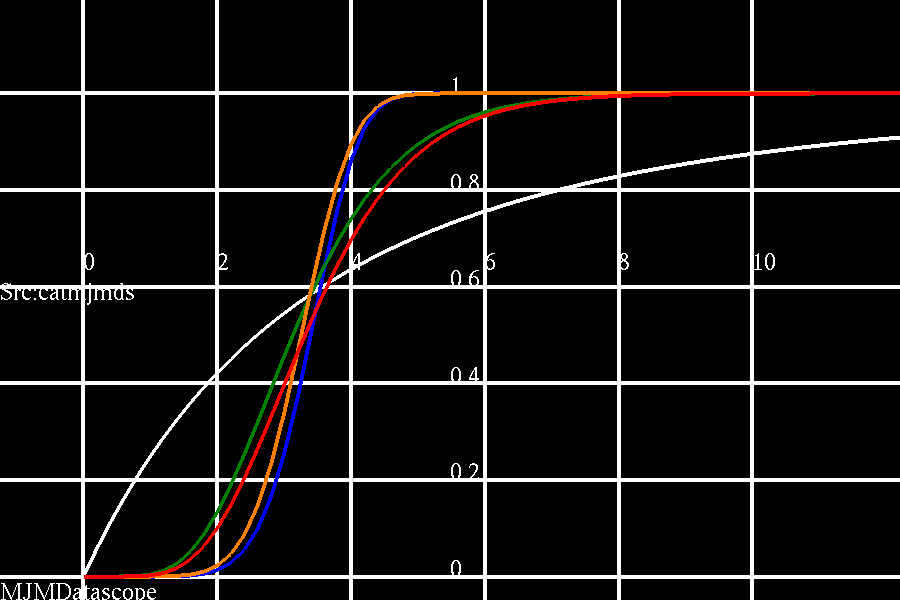
\includegraphics[height=3in,width=4in]{keep/plotleak.png} }
\begin{tabular}{|r|r|r|r|r|r|r|}
\hline
\multicolumn{7}{|c|}{Leaky Response Curve Parameters }\\
\hline
color & n-species &k & exp time & phi-10 & phi-50 &phi-90 \\
\hline
white & 2 &- & .3 & 0.358753 &  2.59927 &  11.5451 \\
green & 10 &0 & 2.75 &  1.85584 &  3.13446 &  5.05911 \\
red & 10 &.5 &  3 &   2.00123  &   3.31509 &  5.24203 \\
orange & 10 &5 &  50 &  2.4503 &  3.25675 &  4.02285 \\
blue  & 10 & 6 &  100 & 2.6079  &    3.39818 &  4.11833 \\
\hline
\end{tabular}
\caption{ Some exposure curves demonstrating less confusion with the loss terms. The y-axis is P of developing while the X-axis is photon flux with exposure time adjusted to get overlapping curves. The exposure time ratio is 333 between 1 photon and the very lossy case. Note that the values here for illustration and may not reflect typial realizable systems of interest  ./plotleak  }
\label{fig:plotleakt}
\end{figure} 
} % mjmpicture
 





\begin{comment}
\begin{table}[H] \centering
\begin{tabular}{|r|r|r|r|r|r|r|}
\hline
\multicolumn{7}{|c|}{Leaky Response Curve Parameters }\\
\hline
color & n-species &k & exp time & phi-10 & phi-50 &phi-90 \\
\hline
white & 2 &- & .3 & 0.358753 &  2.59927 &  11.5451 \\
green & 10 &0 & 2.75 &  1.85584 &  3.13446 &  5.05911 \\
red & 10 &.5 &  3 &   2.00123  &   3.31509 &  5.24203 \\
orange & 10 &5 &  50 &  2.4503 &  3.25675 &  4.02285 \\
blue  & 10 & 6 &  100 & 2.6079  &    3.39818 p&  4.11833 \\
\hline
\end{tabular}

\caption{}
%\label{}
\end{table}
\end{comment}




If this seems familiar its redundant with 
preceding section in mjm\_euv\_multi.tex.
However, the terms are grouped differently to show tri-diagonal
structure and detail the corner cases for small n.
I wrote "mjm\_math" to do a few polynomial manipulations
although it could probably be done in a variety of existing
things like mathematica or sympy. 

\begin{figure}[htb]
\centering

\cee{  X_0 + h$\nu$ -> X_1 }

\cee{  X_{i-1} + h$\nu$ -> X_i }

for i not equal zero or n,

\cee{  X_i ->[k] X_{i-1} }

\mjmeqn{\mjmdt{X_i}=-\phi X_i+\phi X_{i-1} + k X_{i+1}-k X_i 
= \phi X_{i-1} -(\phi + k )  X_i + k X_{i+1} }

otherwise with no decay from terminal state,

\mjmeqn{\mjmdt{X_n}=\phi X_{n-1} }
\mjmeqn{\mjmdt{X_{n-1}}=-(\phi+k) X_{n-1}+\phi X_{n-2}  }
\mjmeqn{\mjmdt{X_0}=-\phi X_0+ k X_{1} }


\caption{ With loss finite lifetime states but stable terminal state . }
\label{fig:leakynrepeat}
\end{figure}

\mjmtol{

wtf n=2,
%\mjmeqn{\mjmdt{X_2}=\phi X_{1} }
%\mjmeqn{\mjmdt{X_{1}}=-(\phi+k) X_{1}+\phi X_{0}  }
%\mjmeqn{\mjmdt{X_0}=-\phi X_0+ k X_{1} }


\mjmeqn{\mjmdtn{2}{X_2}=\phi \mjmdt{X_{1}} }
\mjmeqn{\mjmdtn{2}{X_2}=\left( -(\phi+k)\phi X_{1}+\phi^2 X_{0}   \right) } 
\mjmeqn{\mjmdtn{2}{X_2}=\left( -(\phi+k)\mjmdt{X_{2}}+\phi^2 X_{0}   \right) } 
\mjmeqn{\mjmdtn{2}{X_2}+(\phi+k)\mjmdt{X_{2}}= \phi^2 X_{0}    } 
\mjmeqn{\mjmdtn{3}{X_2}+(\phi+k)\mjmdtn{2}{X_{2}}= \phi^2 \mjmdt{X_{0}  }  } 
\mjmeqn{\mjmdtn{3}{X_2}+(\phi+k)\mjmdtn{2}{X_{2}}
= \phi^2 \left( -\phi X_0+ k X_{1} \right)  }  

\mjmeqn{\mjmdtn{3}{X_2}+(\phi+k)\mjmdtn{2}{X_{2}}
= -\phi^3 X_0+ k\phi \mjmdt{ X_{2} }  }  

\mjmeqn{\mjmdtn{3}{X_2}+(\phi+k)\mjmdtn{2}{X_{2}}
- k\phi \mjmdt{X_{2}}  = -\phi^3 X_0 }  

\mjmeqn{\mjmdtn{3}{X_2}+(\phi+k)\mjmdtn{2}{X_{2}}
- k\phi \mjmdt{X_{2}}  = 
-\phi  \left( \mjmdtn{2}{X_2}+(\phi+k)\mjmdt{X_{2}} \right)
}  
\mjmeqn{\mjmdtn{3}{X_2}+(2*\phi+k)\mjmdtn{2}{X_{2}}
+\phi^2 \mjmdt{X_{2}}  = 0
}  
\mjmeqn{ r(r^2+(2\phi+k)r+\phi^2) =0 }

\mjmeqn{ b^2=4\phi^2+k^2+4k\phi  }
\mjmeqn{ b^2-4ac=k^2+4k\phi  }
\mjmeqn{ r=-\phi-\frac{k}{2} \pm \sqrt{k(k+4\phi)}   }

} % mjtol 


\mjmtol{

 n=3,
\mjmeqn{\mjmdt{X_3}=\phi X_{2} }
\mjmeqn{\mjmdt{X_{2}}=-(\phi+k) X_{2}+\phi X_{1}  }
\mjmeqn{\mjmdt{X_{1}}=-(\phi+k) X_{1}+\phi X_{0}-k X_{2}  }
\mjmeqn{\mjmdt{X_0}=-\phi X_0+ k X_{1} }


\mjmeqn{\mjmdtn{2}{X_3}=\phi \mjmdt{X_{2}} }
\mjmeqn{\mjmdtn{2}{X_3}=\left( -(\phi+k)\phi X_{2}+\phi^2 X_{1}   \right) } 
\mjmeqn{\mjmdtn{2}{X_2}=\left( -(\phi+k)\mjmdt{X_{3}}+\phi^2 X_{1}   \right) } 
\mjmeqn{\mjmdtn{2}{X_3}+(\phi+k)\mjmdt{X_{3}}= \phi^2 X_{1}    } 


\mjmeqn{\mjmdtn{3}{X_3}+(\phi+k)\mjmdtn{2}{X_{3}}= \phi^2 \mjmdt{X_{1}}    } 

\mjmeqn{\mjmdtn{3}{X_3}+(\phi+k)\mjmdtn{2}{X_{3}}= \phi^2 
%\mjmdt{X_{1}}    
\left( -(\phi+k) X_{1}+\phi X_{0}-k X_{2}  \right)
} 

\mjmeqn{\mjmdtn{3}{X_3}+(\phi+k)\mjmdtn{2}{X_{3}}=  
%-\phi^2(\phi+k) X_{1}
-(\phi+k)(\mjmdtn{2}{X_3}+(\phi+k)\mjmdt{X_{3}})  
+\phi^3 X_{0}
%-k\phi^2 X_{2}  
-k\phi \mjmdt{X_{3} } 
} 

\mjmeqn{\mjmdtn{3}{X_3}+2(\phi+k)\mjmdtn{2}{X_{3}}
+((\phi+k)^2+k\phi)\mjmdt{X_{3}})  
=  \phi^3 X_{0}
} 

%\mjmeqn{\mjmdt{X_0}=-\phi X_0+ k X_{1} }
\mjmeqn{\mjmdtn{4}{X_3}+2(\phi+k)\mjmdtn{3}{X_{3}}
+((\phi+k)^2+k\phi)\mjmdtn{2}{X_{3}})  
=   
 -\phi^4 X_0
+ k\phi^3 X_{1} 
} 



} % ssck n=3
\mjmtol{ n==3 part 2

repeat,

\mjmeqn{\mjmdtn{4}{X_3}+2(\phi+k)\mjmdtn{3}{X_{3}}
+((\phi+k)^2+k\phi)\mjmdtn{2}{X_{3}})  
=   
 -\phi^4 X_0
+ k\phi^3 X_{1} 
} 

use identities,
\mjmeqn{\mjmdtn{3}{X_3}+2(\phi+k)\mjmdtn{2}{X_{3}}
+((\phi+k)^2+k\phi)\mjmdt{X_{3}})  
=  \phi^3 X_{0}
} 
\mjmeqn{\mjmdtn{3}{X_3}+(\phi+k)\mjmdtn{2}{X_{3}}= \phi^2 \mjmdt{X_{1}}    } 
\mjmeqn{\mjmdtn{2}{X_3}+(\phi+k)\mjmdt{X_{3}}= \phi^2 X_{1}    } 

\mjmeqn{\mjmdtn{4}{X_3}+2(\phi+k)\mjmdtn{3}{X_{3}}
+((\phi+k)^2+k\phi)\mjmdtn{2}{X_{3}})  
=   
% -\phi^4 X_0
-\phi\mjmdtn{3}{X_3} -\phi 2(\phi+k)\mjmdtn{2}{X_{3}}
-\phi((\phi+k)^2+k\phi)\mjmdt{X_{3}})  
%+ k\phi^3 X_{1} 
+k\phi\mjmdtn{2}{X_3}+k\phi(\phi+k)\mjmdt{X_{3}} 
} 

\mjmeqn{\mjmdtn{4}{X_3}
+(3\phi+2k)\mjmdtn{3}{X_{3}}
+((\phi+k)^2+2k\phi+2\phi^2)\mjmdtn{2}{X_{3}}  
+\phi((\phi+k)^2-k*k)\mjmdt{X_{3}}  
=  0 
% -\phi^4 X_0
%+ k\phi^3 X_{1} 
} 


\mjmeqn{\mjmdtn{4}{X_3}
+(3\phi+2k)\mjmdtn{3}{X_{3}}
%+((\phi+k)^2+2k\phi+2\phi^2)\mjmdtn{2}{X_{3}}  
+(k^2+4k\phi +3\phi^2)\mjmdtn{2}{X_{3}}  
%+\phi((\phi+k)^2-k*k)\mjmdt{X_{3}}  
+(\phi^3+2k\phi^2 )\mjmdt{X_{3}}  
=  0 
% -\phi^4 X_0
%+ k\phi^3 X_{1} 
} 




} % n==3 part2




The characteristic equation then is,

\mjmeqn{\mjmdtn{2}{X_n}=\phi \mjmdt{X_{n-1}} }
\mjmeqn{\mjmdtn{2}{X_n}=
  \phi  \left( -(\phi+k) \mjmdt{X_{n-1}}+\phi \mjmdt{X_{n-2}}   \right) }

\mjmeqn{\mjmdtn{2}{X_n}=
  \phi  \left( -(\phi+k)\mjmdt{X_n}+\phi \mjmdt{X_{n-2}} \right) }

\mjmeqn{\mjmdtn{2}{X_n}=
   -(\phi+k)\phi\mjmdt{X_n}+\phi^2 \mjmdt{X_{n-2}}  }

\mjmeqn{\mjmdtn{2}{X_n}+ (\phi+k)\phi \mjmdt{X_n}
=\phi^2 \mjmdt{X_{n-2}}  }

For n=2, 
%\mjmeqn{\mjmdtn{2}{X_2}+ (\phi+k) \mjmdt{X_2} =\phi^2\left( -\phi X_0+ k X_{1} \right) =-\phi^3 X_0+ k\phi^2 \mjmdt{X_{2}} }
%\mjmeqn{\mjmdtn{2}{X_2}+ (\phi+k) \mjmdt{X_2} =\phi^2\left( -\phi X_0+ k X_{1} \right) =-\phi^3 X_0+ k \phi X_{1} }


\mjmeqn{\mjmdtn{2}{X_2}+ (\phi+k)\phi \mjmdt{X_2}
=\phi^2\left( -\phi X_0+ k X_{1} \right)
=-\phi^3 X_0+ k\phi \mjmdt{X_{2}} 
}


\mjmeqn{\mjmdtn{2}{X_2}+\phi^2\mjmdt{X_2} =-\phi^3 X_0 }

\mjmeqn{\mjmdtn{3}{X_2}+ \phi^2  \mjmdtn{2}{X_2} =-\phi^3 \mjmdt{X_0}
= \phi^4 X_0 - \phi^3 k X_1
 }
\mjmeqn{\mjmdtn{3}{X_2}+ \phi^2 \mjmdtn{2}{X_2} =-\phi^3 \mjmdt{X_0}
= 
% \phi^4 X_0 
- \phi \mjmdtn{2}{X_2} - \phi^3\mjmdt{X_2} 
- \phi^3 k X_1
 }

\mjmeqn{\mjmdtn{3}{X_2}+ (\phi^2+\phi ) \mjmdtn{2}{X_2} 
+ \phi^3 \mjmdt{X_2} 
=- \phi^3 k X_1 = -\phi^2 k \mjmdt{X_2}
 }

%%%%%%%%%%%%%%%%%%%%%%%%%%%%%%%%%%%%%%


\mjmeqn{\mjmdtn{3}{X_2}+ (\phi^2+\phi ) \mjmdtn{2}{X_2} 
+  ( \phi^3 +\phi^2 k) \mjmdt{X_2} =0 
 }


\mjmeqn{ r(r^2+r(\phi+\phi^2)+\phi^2(\phi+k) ) =0 }

\mjmeqn{ b^2=  \phi^2(1+2\phi+\phi^2)  }
\mjmeqn{ b^2-4ac=  \phi^2(1+2\phi+\phi^2)-4*\phi^2(\phi+k)   }



%\mjmeqn{\mjmdtn{3}{X_2}+ (\phi+k-k\phi ) \mjmdtn{2}{X_2} =-\phi^3 \mjmdt{X_0} =-\phi \left( \mjmdtn{2}{X_2}+ (\phi+k) \mjmdt{X_1} \right) }


%\mjmeqn{\mjmdtn{3}{X_2}+ (2*\phi+k-k\phi ) \mjmdtn{2}{X_2} =-  (\phi+k) \mjmdtn{2}{X_2} }










The silver halids
and probably other systems will have more paramter variation and
more physical effects making the equations more complicated. With computers
and numerical codes it may not seem worthwhile to explore these 
analytically but they are useful for early thinking about 
candidate photo systems. 

In a simple  2 photon process a light flux $\phi$ converts A into B
and a potentially different flux or different rate, $\psi$,  converts
B into C. B can also decay back to A. 

\begin{figure}[htb]
\centering

\cee{  A + h$\nu$ -> B }

\cee{  B + h$\nu_2$ -> C }

\cee{  B ->[k_1] A }

\mjmeqn{\mjmdt{A}=-\phi A + k_1 B }

\mjmeqn{\mjmdt{B}=\phi A - k_1 B - \psi B  }

\mjmeqn{\mjmdt{C}=\psi B  }

\caption{ With loss of unstable intermediate B   }
\label{fig:loss} 
\end{figure}

As before variables can be eliminated and a single higher order
linear equation can be solved. 

% showworkcomment
\mjmwork{characteristic eqn }{
\mjmeqn{\mjmdtt{A}=-\phi \mjmdt{A} + k_1 \mjmdt{B} }

\mjmeqn{\frac{1}{k_1}(\mjmdtt{A}+\phi \mjmdt{A}) = \mjmdt{B} }

\mjmeqn{\frac{1}{k_1}(\mjmdt{A}+\phi A )=  B }

\mjmeqn{\mjmdt{B}=\phi A - k_1 B - \psi B  = \phi A -(k_1 + \psi)B }


\mjmeqn{\frac{1}{k_1}(\mjmdtt{A}+\phi \mjmdt{A}) = \phi A - k_1 B - \psi B  = \phi A -(k_1 + \psi)( \frac{1}{k_1}(\mjmdt{A}+\phi A )) }
\mjmeqn{\frac{1}{k_1}(\mjmdtt{A}+\phi \mjmdt{A}) =  \phi A -(k_1 + \psi)( \frac{1}{k_1}(\mjmdt{A}+\phi A )) }

\mjmeqn{\frac{1}{k_1}\mjmdtt{A} +\frac{1}{k_1}\phi \mjmdt{A} =  (\phi-\frac{\psi\phi}{k_1} -\phi ) A -(k_1 + \psi)\frac{1}{k_1}\mjmdt{A}  }

\mjmeqn{\frac{1}{k_1}\mjmdtt{A} +(k_1 + \psi+\phi)\frac{1}{k_1}\mjmdt{A}  + \frac{\phi\psi}{k_1} A  = 0 }

\mjmeqn{\mjmdtt{A} +(k_1 + \psi+\phi)\mjmdt{A}  +\phi\psi   A  = 0 }

\mjmeqn{r = -\frac{(k_1 + \psi+\phi)}{2}  \pm \frac{1}{2}\sqrt{(k_1+\psi+\phi)^2 -4\phi\psi }  }


\mjmeqn{r = -\frac{(k_1 + \psi+\phi)}{2}  \pm \frac{1}{2}\sqrt{k_1^2+2k_1*(\phi+\psi) +(\psi+\phi)^2 -4\phi\psi }  }

\mjmeqn{r = -\frac{(k_1 + \psi+\phi)}{2}  \pm \frac{1}{2}\sqrt{k_1^2+2k_1*(\phi+\psi) +(\psi-\phi)^2  }  }

} % mjmwork
Its probably worth nothing that the earlier system had degenerate roots
and this one may approach that.  Consider two roots r and $(r+\delta)$
and pairs of  constants $A_x$ and $A_y$ defined below. 
In the limit of small $\delta t $ the exponential can be expanded
although for finite $\delta$ this will always grow with time.

% showworkcomment
\mjmwork{degenerate roots }{
\mjmeqn{ A= A_-e^{rt} + A_+e^{(r +\delta)t  } ;
\mjmdt{A} = A_-re^{rt} + A_+(r+\delta)e^{(r +\delta)t}}

\mjmeqn{ A(0)= A_- + A_+ ;  
\mjmdt{A}(0) = A_-r + A_+(r+\delta)=-\phi A(0)}

\mjmeqn{ rA(0) + A_+\delta = - \phi A(0) }
\mjmeqn{ (\phi + r)A(0) =- A_+\delta } 
Using "engineering ( aka gutter ) math" take limit as delta goes to zero,

\mjmeqn{ A= e^{rt}(A_z + A_d(1+\delta t))  } ;
change variables, 
} % degenerate roots 

The general solution can be written as, 
\mjmeqn{ A= e^{rt}(A_1 + A_2\delta t)  } ;
with 
\mjmeqn{ \mjmdt{A}= e^{rt}( A_2\delta+ rA_1+rA_2\delta t )  } ;
and its possible to solve for $A_2\delta$ product,
\mjmeqn{ A(0)= A_1 } ;
\mjmeqn{ \mjmdt{A}(0)= (  rA(0)+A_2\delta(1+0) )  } ;
\mjmeqn{ A_2\delta= \mjmdt{A}(0)- rA(0)  } ;
or   
\mjmeqn{ A= e^{rt}(A(0) + (\mjmdt{A}(0)-rA(0)) t)  } ;

In any case the discriminant is positive semidefinite and 
an osillatory response is not possible. 




\subsection{ Simultaneous Multi-photon Absorption  }

One point of this work is to use the multi-photon term 
for processes such as the above although in general usage for
EUV it seems to be specialized to simulateous absorption
of n-photons or proceeeding through virtual states. 
As shown in the previous section, the temporal correlation 
related to the leaky integration helps to sharpen the curve
and in fact the simultaneous curve does appear to have a
smaller zone of confusion than the long lived intemediate state
case for same number of required photons but of course it
wastes more. 

\begin{figure}[htb]
\centering

\cee{  A + nh$\nu$ -> B }


\mjmeqn{ \mjmdt{A} =   -A \phi^n }  
\mjmeqn{ \mjmdt{B} =   A \phi^n }  
\mjmeqn{A(t)=A(0)(exp(-\phi^n  t )) }

\mjmeqn{ \mjmdt{B} =   \phi^n A(0)(exp(-\phi^n  t )) }
\mjmeqn{ B(t) =   A(0)(1-exp(-\phi^n  t )) }

\mjmeqn{ B(\phi;t) =   A(0)(1-exp(-\phi^n  t )) \label{eqn:simultaneous} }

versus 

\mjmeqn{ X_{n} = X_0(0)( 1- \exp(-\phi t) \sum_0^{n-1} \frac{(\phi t)^i}{i!}  ) \label{eqn:multipagain} }

\caption{ Multiple photons per simultaneous reaction  generate \mjmrefeqn{simultaneous} versus \mjmrefeqn{multip} reproduced here as \mjmrefeqn{multipagain} without the constant.     }
\label{fig:simultaneous} 
\end{figure}
Note that these are all exponential in time but for a given scene
at fixed time the exposure curve $B(\phi)$ does become sigmoidal
and 

\mjmeqn{ \mjmdphi{B(\phi;t)} =   tn\phi^{n-1}exp(-\phi^n  t )) }
with n-1 zero derivatives at zero light levels.
With second derivative($n>1$), 
\mjmeqn{   (-t^2n^2\phi^{2n-2}+tn(n-1)\phi^{n-2})exp(-\phi^n  t )) }
the maximum slope appears at  
\mjmeqn{ t=\frac{n-1}{n}\phi^{-n} }
with value 
\mjmeqn{ \mjmdphi{B(\phi;t)}_{max} =   tn\phi^{n-1}exp(-\phi^n  t ))= (n-1)\phi^{-1}exp(-\frac{n-1}{n} )), n>1  }

\mjmtol{check this lol }
The $n=1$ result does not seem right but the max is at $\phi=0$, 
\mjmeqn{ \mjmdphi{B(\phi;t)}_{max} = t exp(-\phi  t )= t  }

Comparing  \mjmrefeqn{simultaneous} to \mjmrefeqn{multip} or \mjmrefeqn{multipagain}, the lack of time integration is obvious from the apprerance of t to first power only. 

 

\mjmpicture{plotsimu.png}{  Multi-photon simulatnaous for t=n=1(green),2(white),3(blue),and 5(red). Time was set equal to photon number to make curves overlap better to show relative shapes. ./plotsimul  }{pseudo}

%\mjmpicture{plotsome.png}{Multiphoton scaled and translated to intersect at .5 . Illustrated are 1,2,3,4, and 101 photon curves. plotsome.txt }{scaledmulti}



\subsection{ Multi-step or maybe pyramind }
A differnt example more similar to "multi-trigger" imaging gives the
same result.
Consider the system and  rate equations in \mjmreffig{pyramid},

\begin{figure}[htb]
\centering

\cee{  A + h$\nu$ -> B }

\cee{  nB ->[k] C }

\mjmeqn{ \mjmdt{A} =  - A \phi }  

\mjmeqn{ \mjmdt{B} = -\mjmdt{A}-\mjmdt{C}=  A\phi -  n k B^n  }  
\mjmeqn{ \mjmdt{C} =  k  B^n  }  


\caption{ Multi-step or pyamid }
\label{fig:pyramid} 
\end{figure}


with initially A(0)=$A_0$ and B(0)=0.
\mjmeqn{A(t)=A(0)(exp(-\phi t )) }
giving 
\mjmeqn{ \mjmdt{B} = \phi A(0)exp(-\phi t ) -  k  B^n \label{eqn:pyr}  }  

With the developer responding to $[C]$ the response curve does have
n zero derivatives at the origin as B(0) is zero but the details
are different. B responds more quickly as its first order but then
there is a long tail in C as B is depleted. 
Changing $k$ from unity can help. 
To modify this system
to copy the Poisson n-photon results?  


\mjmtolx{ I never could get the right form yet, doesn't work on this system

Guessing the solution again,
\mjmeqn{ C(t) = A(0)\phi( 1- \exp(-\phi t) \sum_0^{n-1} \frac{(\phi t)^i)}{i!}  ) }
\mjmeqn{ \mjmdt{C} =  A(0)\phi  \exp(-\phi t)  \frac{(\phi t)^{n-1})}{(n-1)!}   }
\mjmeqn{ \mjmdt{B} =  A(0)\phi  \exp(-\phi t)( 1 -  \frac{(\phi t)^{n-1})}{(n-1)!})   }


can be verified easily with properties outlined before. ,
}


\mjmpicture{pyramid_bad.png}{ Some miscellaneous pyramid transfer curves including some with decay of B back to A. The initial zero derivative could be demonstrated but the slope through transition region was comparatively low and asymptotes were usually less than 1.  $  ./mjm_poisson.out "test test=pyramid;n=10;dt=.00001;time=.001;k=100;phi=.0;dphi=5;nphi=1000;color=white;itaut=100" quit $ }{pyramidcurves}


 








The resolution and fluctuatin properties of multi-photon
processes are also beneficial.




\subsection{Some EUV Resists - CAR and MTR etc}

\subsubsection{Chemically Amplified  }

Several good reviews exist
\cite{Ito_Chemical_Amplification_Resists_2005}.
The important points which can be found detailed in most
references relate to multiple chemical reactions in response to
one photon. 
As usually used in the field, chemically amplified resists
sense UV light with a photoacid generator(PAG) and use the
generated acid to catalytically remove groups from a 
polymer. Polymers with enough removed groups are lost
during development.  PAG's appear to commonly use sulfur species.
The "deprotection" scheme is common although polymerization and
depolymerization are also possible. 

A 2022 review compared some CAR's, MOR's, and MTR with an EUV interference
grating illumination pattern demonstrating some benefits of the MTR 
method although all resits had some limitations
\cite{DouglasGuerreroadditionalGillesRAmblard_lithography_resist_2023}.
Interfernce between plane waves would generate a sinusidal intensity
profile and the resulting intensity profile is claimed as
sinusoidal. In any case the line
edges will not be digital or "sharp" and have some profile 
although in actual lithography this may be different and variable
the resist with a high-contrast transfer function may have 
noise benefits. The spatial frequencies or other parameters of the
noise may not be evident and problems like diffusion will not
be considered but sharp transitions create a better starting point
than exponential or gradual ones. 

Attempts to optimize resist parameters for EUV have not always
produced the expected results. A 2018 attempt to add proprietary Mg
and related salts as sensitizers actually decreased EUV absorption
and largely increased roughness while increasing acid generation
and apparent electron generation
\cite{Vesters_Jiang_Yamamoto_Sensitizers_extreme_ultraviolet_2018}.
The ability to change the electron-hole pair generation energy,
usually estimated using Klein's 3x the bandgrap rule in semoconductors,
creates some interesting possibilities although impoved photon
efficiency would probably help quanizatin problems more.

More recently around the turn of the century, some benefits were
observed with Sn in the right environment without amplification
\cite{Belmonte_Cendron_Reddy_Mechanistic_insights_2020}.


In the prior curves, "photon" was used as a generic term
but in reality reactions could be initiated by electrons
fron an initial absorption event or from the ambient.
A background of ions may exist which could create a uniform
fog or exposure and a multi-event resist may be able to
avoid some of this pattern deterioration. 





\subsubsection{Multi-trigger }

Multi-trigger resists appear to be the closest thing to
the multi-photon idea applied to DUV or EUV lithigography.
A 2018 paper describes the concept as spec
"The multi trigger
resist (MTR) is a negative tone crosslinking resist that does not need a post exposure bake
(PEB)"
but gets to multi event property
"e reaction will only proceed where
an MTR molecule and a crosslinker are
simultaneously activated in close proximity to each
other"
\cite{Popescu_Vesters_McClelland_Multi_Trigger_Resist_2018}
although this work does not appear to show any rate equations or
characteristic curves.

\mjmtol{ make sure to come back after doing CAR as the acid 
dynamics are unclear among other possible problems with the words.}

A later paper 
\cite{RoelGronheidadditionalDanielPSanders_Multi_trigger_resist_novel_2019}
described some resist design considerations, "
resolution, line edge roughness and sensitivity requirements, 
with minimal defectivity. However, these parameters
are linked by a fundamental trade-off in lithography (the RLS triangle)
and it is difficult to overcome. For instance, addition of quenchers in
chemically amplified resists (CAR) reduces the acid diffusion length and
increases the resolution of the patterned features, but decreases the sensitivity,
and impacts on material stochastics affecting the line edge roughness. Defectivity
due to line collapse, bridging or line breaks is also a fundamental problem."
 
The authors go on to illustrate the concept with pictures although no
obvious reactions or rate equations.  From the pictures, the reaction
sequence may be, 

\cee{X + $h\nu$ -> P } 

\cee{A ->[P] $A^\prime$ } 

\cee{B ->[P] $B^\prime$ } 

\cee{$A^\prime +B^\prime$  -> C  } 

With C being the developer selectivity component.
Rate equations would then be,

\mjmeqn{ \mjmdt{X}= -\phi X }

\mjmeqn{ \mjmdt{P}= -\mjmdt{X} }

\mjmeqn{ \mjmdt{A}= -  A P ;  \mjmdt{A^\prime}= A P - \mjmdt{C} }

\mjmeqn{ \mjmdt{B}= -  B P ; \mjmdt{B^\prime}= B P- \mjmdt{C} }

\mjmeqn{ \mjmdt{C}= A^\prime B^\prime }

X and P are straightforward,

\mjmeqn{ X= X_0 exp(-\phi t) }
\mjmeqn{ P= X_0(1- exp(-\phi t)) }
with A and B being identical but more complicated,
\mjmeqn{ \mjmdt{A}= -  A X_0(1-exp(-\phi t))   }
\mjmeqn{ -ln(A) =  X_0(t+\frac{1}{\phi}exp(-\phi t))+c   }
\mjmeqn{ ln(A) =  X_0(-t-\frac{1}{\phi}exp(-\phi t))+c   }

\mjmeqn{ A =  A_0exp(-X_0 (t-\frac{1}{\phi}(1-exp(-\phi t))))   }
as $\phi$ goes to zero this seems to have the right limit,

\mjmeqn{ A \approx  A_0exp(-X_0 (t-\frac{1}{\phi}(\phi t)))   }

Under these conditions A and B are identical leading to

\mjmeqn{ \mjmdt{A^\prime}= A P - (A^\prime)^2 }
\mjmeqn{ \mjmdt{A^\prime}= 
A_0X_0exp(-X_0 (t-\frac{1}{\phi}(1-exp(-\phi t))))(1- exp(-\phi t)) 
- (A^\prime)^2 }

\subsection{Multi-trigger with quencher }

Perhaps a little more accurately, consider the system
with X and Z dead or inactive components, 


\cee{A + $h\nu$ -> A^* } 

\cee{Q + $h\nu$ -> X } 

\cee{A^*  -> A } 

\cee{A^* + Q -> Z } 

with the final polymerization step being left vague as issues
with strnaded monomers and crosslinking are ignored right now, 

\cee{M+P ->[A^*] P } 

\cee{M+M ->[A^*] P } 

Taking the last process first, assume that a monomer can be attached
to anything anywhere and that P regardless of shape or length
is left after development,  

\mjmeqn{ \mjmdt{P}= A^* M  }

\mjmeqn{ \mjmdt{M}= -  A^* M  }

The others are straightforward,

\mjmeqn{ \mjmdt{A}= -A\phi  }
\mjmeqn{ \mjmdt{Q}= -Qk_q\phi  }

\mjmeqn{ \mjmdt{A^*}= A\phi  -\frac{1}{\tau} A^* -Q A^* }


initial amounts of A,Q, and M are present and maybe drop time
constant.  As with other cases,
\mjmeqn{ A(t) = A_0exp(-\phi t)  }
\mjmeqn{ Q(t) = Q_0exp(-k_q\phi t)  }

\mjmpicture{quench.jpg}{ The quencher is paramterized to be destroyed before the catalyst is activated and destriryed. The initial slope should be zero but if the catalyst is depleted the final amount of polymer is limited below 1.  $  ./mjm\_poisson.out "test test=mtrigq;a0=5;tau=10;phif=10;q0=100;t=1;kq=20;dt=.001" quit  $ }{quench}




\mjmeqn{ \mjmdt{A^*}= \phi A_0exp(-\phi t)
				-Q_0exp(-\phi t) A^*   -\frac{1}{\tau} A^*  }
Using an integrating factor,
\mjmeqn{ F = (\int ( Q_0exp(-\phi t)+\frac{1}{\tau})dt)   }
\mjmeqn{ F = (-\frac{ Q_0exp(-\phi t)}{\phi}+\frac{t}{\tau})  }

\mjmeqn{A^* = exp(-F)\int(exp(F)A_0exp(-\phi t) dt) + C exp(-F) }
The integral may be doable,

\mjmeqn{I = \int(exp( -\frac{ Q_0exp(-\phi t)}{\phi}+\frac{t}{\tau}) A_0exp(-\phi t) dt) }


\mjmeqn{I_t = \int(exp( -\frac{ Q_0exp(-\phi t)}{\phi}+\frac{t}{\tau})
(  A_0exp(-\phi t)+\frac{A_0}{Q_0\tau}) dt) }

\mjmeqn{\frac{d}{dt} (exp( -\frac{ Q_0exp(-\phi t)}{\phi}+\frac{t}{\tau}))
= (Q_0exp(-\phi t) +\frac{1}{\tau}) exp(F)  
}

\mjmeqn{I_t = \frac{A_0}{Q_0}exp(F)}







\section{Silver Halides}

Despite their long history of usage in applications ranging 
from consumer imaging to X-ray and astronomy applications,
 a lot remains unknown about the
details of latent or developed image formation in silver halide films.
A 1980 review did suggest the in real films it took about 4 photons to
create an image by a process involving atom motion \cite[p. 229]{Bose1980} .
Several other short reviews exist highlighting other aspects
such as grain properties and amplification by up to $10^9$
\cite{Tan_Silver_Halides_Photography_1989}.


A turn of the century conference paper reviewed the history and basis
for 1,2, and 4 photon mechanisms \cite{DBLP:conf/pics/Leubner99} with
the stated interest of optimizing a one photon process due to efficiency.
\mjmtol{ The author mentions Tani who did suggest 2 photon processes
suppress dark current. Most solid-state electronic imagers are one photon and have good efficncy as well as linearity but also huge dark current which may be a consequence of this mechanism although need to check the numbers }
The author outlines a system similar to the cascade above with
each photon ( equivalent to an electron here ) adding to a growing
neutral silver cluster,

\newcommand{\mjmcee}[2]{{\centering { \cee{#1 \label{#2} }}}}

\mjmcee{  Ag_n + Ag^+ + e^-  -> Ag_{n+1} }{eqn:halides}
%\cee{  X_n + h$\nu$ -> Ag_{n+1} }

n=4 is thought to be stable and developable while smaller clusters
can decay or fail to develop.  The net equation is then

\cee{  4Ag^+ + 4e^-  -> Ag_{4} }


A two photon process is also described where photo generated holes
are converted to electrons but this seems to rely on existing
$Ag_2$ clusters that either already exist or were photogenerated earlier,

\cee{  2Ag_2(H) +  2h^+  -> 4Ag_{4} + 2e^- }

or

\cee{  2Ag^+ + Ag_2 + 2e^-  -> Ag_{4} }

In considering a one photon process, the author tries to distinguish
optical and thermal processes, " This one-photon process thus needs 
light exposure
to provide both the electron and the hole and is not triggered 
by thermal electron or hole events."
Although no idea what this means. In any case, a one photon process
was considered using "reduction sensitization centers" or similar
electron traps. These mechanisms reduce to
\mjmcee{ h\nu + 2Ag_2 ->Ag_4}
or with the use of Au,
\mjmcee{AuAg_3^+ + e^- -> AuAg_3 }
The former equation is thought to have a photon threshold around 1.4eV
which the author notes is well above thermal voltages suggesting no
dark current but this misses important issues. In any case it is many
thermal voltages ( typically taken as 26meV not the 30 given here ) 
above the silicon band gap and band-to-band generation may be less
for similar quantum efficincies.\mjmtol{ "do the math" somewhere } 




\subsection{Notable featues Silver Halides} 

Superionic conducitivity in AgI 
\cite{Carvalho_Negi_Neto_Direct_calculation_2022} 
which apparently is equivalent to the  
 existence of a Hall Mobility
\cite{Liou_Hudson_Wonnell_Ionic_Hall_effect_1990}
. It appears to persist
in compounds such as $C_5H_6NAg_5I_6$ \cite{Newman_Frank_Matlack_ionic_hall_effect_1977}.


\subsection{Silver Bromide solid} 





Copper sulfides can form varying large unit cell crystals
with correrpsondingly high integer stoichiometry.
They apparently are not molecular crystals.
Unit cells may contain 24 or 62 distinct copper atoms and some phases
contain a sulphur HCP structure with interstial Cu that become
fluid above 100C \cite{Evans_crystal_structures_}.







\section{X-ray detectors }

The EUV has been studied some what but a lot more literature
exists on X-ray detectors. While soft X-rays may be somewhat
similar to EUV, even the harder X-rays will explore relevant
part of the materials including core electrons that may 
ignored in lower energy studies. This may be important as
core electrons and relativistic effects have recently been shown
to be important contributors to the potential of the lead
acid battery and liely effect EUV resist physics and cheisty.

Halide perovskites are one class of X-ray detector
with a recent interest in lead-free versions
\cite{doi:10.1021/acsaom.4c00265}.









While silver halide literature for nm scale patterning is scarce,
there is experience with some pieces. For example, submircon silver
clutsters were formed in a mixture of silver and PMMA
\cite{PMC4820741}.


AgBr captures the "hole" to make Br and Ag both neutrals and the
hole can escape as a gas. 

One step in the cluster formation may involve atom migration.
The relevance to dark "current" or exposure needs to be considered
but also any relevance of the primary EUv energy on related
processes. 


\subsection{sulfur}

fluidd copper phase in hcp S lol 
MoS

\subsection{Non-local : grad, erode, dilate, etc }


\subsection{"Move Towards the Light" the EUV Litho Near Death Experience}

While diffusion seems to be inescapable part of photoresist mechanism
ion or atom aggregatopm does not seem motivated although it
is central to the notions of silver halide latent image formation.











\section{Early Events and Ultimate Fate }

One important aspect of the lithographic process is
the early steps in converting the photon into
a latent image. Two processes are commonnly considered.
The more common involves creation of a single electron 
which may thermalize much later. Alternatively several 
electrons could be created almost simultaneously from
the same atom.
With the interest in metal oxide resists and the topic
of this work being largely silver halides, details of
absorption in metals such as silver and tin may be useful
to describe and compare where known. 

Silver is the immediate issue but tin is of importance
too. It appears there are a lot of small issues that likely
matter to simple macroscopic results. 
Its worth noting that just recently the potential of the lead
acid battery was explained by adding relativistic terms to 
the pseudopotential for the valence states
\cite{Ahuja_Blomqvist_Larsson_Relativity_Lead_2011}.
The authors contrast lead to tin by the nuclear charge and
then attribute several properties to the additional
relativistic effects. Core electrons differ between
elements placing different contstraints on outer
shell behavior. 


Due to the participation of possibly lower level shells in
relevant transitions, some DFT pseudopotential calculations
may be limited. A variety of specialized techniques exist
that may provide details on initial EUV-resist interaction.
A Lanczos theory applied to inner shell absorption and photoionization
was recently published
\cite{Moitra_Coriani_CabralTenorio_Inner_shell_photoabsorption_2021}.
Variations on the EOM-CCSD method exist such as an
STEOM  or similarity transformed approach \cite{doi:10.1021/acs.jctc.4c01181}.
One problem seems to be dealing well with the continuum free states
which is addressed by several methods
\cite{doi:10.1021/acs.jctc.1c00303}.

Tables of element EUV absorption coefficients have produced
and show several metals including Sn, Sb, Ag, Cs, Bi, Pb have
comparably high molar absorption rates  along with I 
\cite{PMC11433861}. Translation into resist performance of course
is complicated by chemical environment and actual fate of the
absorbed light energy. Paradoxes and surprises have been observed
as mentioned elsewhere. As some resists molecules have dimensions 
approaching the light wavelength especially with a high dielectric constant
various "particle in a box" or antenna effects may be considered.
Quantum effects and relativity probably dominate.  

A study of oxo caged tin and tin butyl clusters below 70 ev
demonsrated a negative tone resist with exposed areas losing
organics \cite{PMC10926160}. The later discussion of Sn-butyl
clusters is vaguely similar to the issues with silver halide
clusters although many specific are different. 

While not directly applicable to photoresist design, a lot 
of work over the last few decades
 has explored the photocathode properties of some 
materials containing high absorption elements.
A 1996 work looked at stability and quantum efficiencies
of materials such as metal halides such as AgCl and CsI
into the 1 nm range
\cite{OswaldHWSiegmundfirstMarkAGummin_title_Progress_1996}.
While there was a significant angle dependence of emission
its not clear how the test geometry influenced this and
if it is relevant at all to photoresist under high NA exposures.
Resists would generally want to minimize electron emission
and instability may indicate latent image formation.
Although if the emitted electron does not cause exposure
of random resist, the charging of the exposed region could
cause a variety of other effects. 




A 2025 work discusses some EUV resist issues and results with silver
and gold dry-develop resists with n-heterocycle complexes
\cite{https://doi.org/10.1002/smll.202407966}. While one gold resist
was ultimately selected for further evaluation, a neglected story
may exist in their figure 2c. In these 3 eposure curves 2 appear
more or less exponential while the third one, with 2 Ag centers
denoted (i-Pr)L-AuCl demonstrated no response below a threshold of 
about 100mj/cm2 followed by a concave downward ( like $e^n, n<1$ ) 
approach to 1. The authors subsequently dismiss this resist as the
PF6 provides better sensitivity. It would be interesting to look at
the initial part of these curves to see if there is an observable
delay period. Simple "sensitivity" issues should not cause
a dealy but rather an exponential over a longer dose range.
\mjmtol{ Also they elaborate on electron thermalization with nice pictures
but AFAICT this is really an unknown and needs to be investigated.  
I became aware of how glib some filler material is from the medial
literature. Someone probably said it and it is plausible but
never verified although the details here could be important. }


As early as 2022 good reviews exists on metal containing
e-beam resists with possible utility for EUV. For example,
Saifullah et al consider self-developing metal oxide and halide
resists and discuss less known mechanisms such as Knotek-Feibelman
which can create 3 electrons on impact
\cite{Saifullah_Tiwale_Ganesan_Review_metal_containing_2022}.
They go through metal sulfoxide resists characteristic curves
exhibiting a threshold charge dose to begin developing a latent image.
Silver is mentioned in passing but not as a halide.

It turns out that lead halides and related perovskites containing
organics have been investigated for photovoltaic performance
that provides some information on EUV issues.
One recent work suggests they have a lot of remarkable
properties  and go on to do some analysis in the EUV region
\cite{Green_Jiang_Soufiani_Optical_Properties_Photovoltaic_2015}.
While the goals of these efforts are to produce stable energy
sources, their susceiptibility to decomposition under illumination
is exactly a desired feature of a photoresist. 
Both lead and iodine have decent EUV absorption and the possibilities
of designing conversion of light into decomposition may be worth
exploring. 

Its also worth keeping in mind while exploring resist candidates that
the resist itself could form the desired features such as conductors.
This process has been explored in a set of techniques called direct
optical lithogrphy\cite{D4TA06618A}. As several resists begin with
metal compounds that become more metallic in exposed areas the
potential is there to directly form condcutors.  

An earlier thesis from 2016 explored an HfO resist which appeared
to use sulfate to control aggregation 
\cite{Luo_Deposition_characterization_patterning_2016}.
The resist was also explored for response to electrons and found
to response to energies as low as 2eV with a high enough dose
although later XPS analysis of sulfur content suggests some details
need to be explored.
A 30kev He+ ion beam was also found to work with 50-100 times
more sensitivity than 30kev electrons. In the reiew of past methods,
this thesis also mentions $Ag_2S$ and similar resists and their
limitations.  






\section{Conclusions}

\section{Supplemental Information}

\subsection{Computer Code}


\begin{lstlisting}

picture from datascaope, 

 2068  ./mjm_poisson.out -cmd "plot 0 10 .1 3 3" -cmd quit
 2069  ./mjm_poisson.out -cmd "plot 0 10 .1 30 3" -cmd quit
 2070  ./mjm_poisson.out -cmd "plot 0 100 .1 30 3" -cmd quit
 2071  ./mjm_poisson.out -cmd "plot 0 10 .1 1 3" -cmd quit
 2072  history


\end{lstlisting}
\section{Bibliography}


\bibliography{\mjmbasename,\mjmaddbio,../copper/copper}
\bibliographystyle{plainurl}


%%%%%%%%%%%%%%%%%%%%%%%%%%%%%%%%%%%%%%%%%%%%%%%%%%%%%%%%%%%%%%%%%%%%%%%%%%%%%
\begin{acknowledgments} 

% \input{generalack.tex}
\begin{enumerate}
\item Pubmed eutils facilities and the basic research it provides. 
\item Free software including Linux, R, LaTex  etc.
\item Some discussion with Frederick Chen   on Linked In \cite{Chen_Chen_Chen_Kaohsiung_City_Kaohsiung_City_2025}.
\item Some discussion with Alex Robinson \cite{Robinson_West_Midlands_England_United_2025}
\item Thanks everyone who contributed incidental support. 
\end{enumerate}

\end{acknowledgments}

%%%%%%%%%%%%%%%%%%%%%%%%%%%%%%%%%%%%%%%%%%%%%%%%%%%%%%%%%%%%%%%%%%%%%%%%%%%%%
\clearpage
\appendix

\begin{mdpicomment}

\section{ Statement of Conflicts }
 No specific funding was used in this effort and there are no relationships
with others that could create a conflict of interest. I would like to develop
these ideas further and have obvious bias towards making them appear 
successful. Barbara Cade, the dog owner, has worked in the pet food industry
but this does not likely create a conflict. We have no interest in the
makers of any of the products named in this work.  

\end{mdpicomment}

\begin{mdpicomment}
\section{About the Authors and Facility}
This work was performed at a dog rescue run by Barbara Cade and
housed in rural Georgia.  The author of this report 
,Mike Marchywka,
has a background in electrical engineering and 
has done extensive research using free online literature sources.  
I hope to find additional people interested in critically 
examining the results and verify that they can be reproduced
effectively to treat other dogs.

\begin{comment}
\begin{figure}[htb] 
\centering
\mjmed{ picture commented out to save space in drafts...  } 
%\includegraphics[width=\picwidth]{me_on_brick.jpg}
\caption{ 
 }
\end{figure}

\end{comment}

\section{ Some Math Stuff }



Bimolecular recomination for example,

\mjmeqn{ \mjmdt{A} = A-A^2}

you can guess something like
\mjmeqn{A=\frac{1}{t+f} }
and get
\mjmeqn{\mjmdt{f}=-(t+f) }
which can be solved with an integrating factor
giving
\mjmeqn{A=\frac{1}{1+Ce^{-t}} }

actually better was partial fractions ,

\mjmeqn{ \frac{dA}{A(1-A)} = dt }
leading to same results doh.





\section{Symbols, Abbreviations and Colloquialisms}

\begin{comment}
% grep "[A-Z][A-Z]" paradox.tex | sed -e 's/[^A-Z]/\n/g' | grep "[A-Z]" | sort | uniq -c
% cat  paradox.tex | sed -e 's/  */\n/g' | grep "[A-Z][A-Z]"  | grep -v "[^A-Z]" | sort | uniq  |awk '{print $0" &   \\\\"; }'
\end{comment}


%\abbreviations{The following abbreviations are used in this manuscript:\\
%\begin{table}
\noindent
\begin{tabular}{@{}ll}
%SMVT & Sodium dependent Multi-Vitamin Transporter\\
TERM & definition and meaning   \\
\hline
%TLA & Three letter acronym\\
%LD & linear dichroism
\end{tabular} % }
%\end{table}

% https://tex.stackexchange.com/questions/5957/bibtex-entry-for-white-papers-and-technical-reports

\section{General caveats and disclaimer }
\label{appendix:caveats}

%\input{disclaimer-informal.tex}

This document was created in the hope it will be interesting to
someone including me by providing information 
about some topic that may include personal experience or a literature
review or description of a speculative theory or idea.
There is no assurance that the content of this work will be
useful for any paricular purpose. 
%In no case am I claiming to provide useful advice on any matter
%but attempting to describe events in terms of literature known
%to me. 


All statements in this document were true to the best of my knowledge
at the time they were made and every attempt is made to assure
they are not misleading or confusing. However, information provided by
others and observations that can be manipulated by unknown causes  
( "gaslighting" ) may be misleading. Any use of this information should
be preceded by validation including replication where feasible.
Errors may enter into the final work at every step from conception
and research to final editing. 
%No assurance can exist that obvious conclusions will be useful
%and may be misleading. 



Documents labelled "NOTES" or "not public" contain
substantial informal or speculative content that
may be terse and poorly edited or even sarcastic or profane.
Documents labelled as "public" have generally been edited
to be more coherent but probably have not been reviewed
or proof read. 

Generally non-public documents are labelled as such to avoid
confusion and embarassment and should be read with that understanding.


\section{Citing this as a tech report or white paper }
\label{appendix:citing}

Note: This is mostly manually entered and not assured to be error free.

This is tech report \mjmtrno. 

\begin{table}[H] \centering
\begin{tabular}{r|r|c|r}
Version & Date & Comments  &  \\
0.01 & \mjmmakedate  &  Create from empty.tex template  &  \\
-  & \today & version  \mjmversion { }   \mjmtrno  &  \\
1.0 & 20xx-xx-xx & First revision for distribution &  \\
\end{tabular}
\end{table}


Released versions,

build script needs to include empty releases.tex
\begin{table}[H] \centering
\begin{tabular}{|r|r|l|}
Version & Date & URL    \\
\hline
\expandableinput{releases.tex}
\hline
\end{tabular}
\end{table}





% 2020-11-30 keep on same page 
%\input{bibtex2.txt}

\begin{minipage}{\linewidth}
%\input{bibtex2.txt}
%\input{bibtex3.txt}
\mjmshowbib
\end{minipage}




\begin{comment}

\end{comment}
\vspace{1cm}
Supporting files. Note that some dates,sizes, and md5's will change as this is
rebuilt.

This really needs to include the data analysis code 
but right now it is auto generated picking up things from prior
build in many cases 
\lstinputlisting{\mjmbasename.bundle_checksums}
\end{mdpicomment}
\end{document}
